\section{Incompressible Navier-Stokes Solver}
\label{IncNSsolver}

\newpage
3.4/UserGuide/Tutorial/IncNavierStokesSolver/Stability
3.4/UserGuide/Examples/IncNavierStokesSolver/Adjoint
3.4/UserGuide/Examples/IncNavierStokesSolver/Aorta
3.4/UserGuide/Examples/IncNavierStokesSolver/Biglobal
3.4/UserGuide/Examples/IncNavierStokesSolver/Direct
3.4/UserGuide/Examples/IncNavierStokesSolver/KovasznayFlow2D
\subsection{Synopsis}
\subsubsection{Velocity Correction Scheme}
\label{VCSscheme}
A useful tool implemented in Nektar++ is the incompressible Navier Stokes solver that allows to solve the governing equation for viscid Newtonians fluid using two different algorithms. 

\begin{subequations}
\begin{equation}
   \frac{\partial \mathbf{V}}{\partial t} + \mathbf{V} \cdot \nabla \mathbf{V} = -\nabla p + \nu \nabla^2 \mathbf{V} + f
 \end{equation}
 
 \begin{equation}
    \nabla \cdot \mathbf{V} = 0
    \end{equation}
 \end{subequations}
 
where $V$ is the velocity, $p$ the pressure and $\nu$ the kinematic viscosity. The first approach uses a splitting/projection method where the velocity matrix system and the pressure are typically decoupled. Splitting schemes are typically favourite for their numerical efficiency since for a Newtonian fluid the velocity and pressure are handled independently, requiring the solution of three (in two dimensions) elliptic systems of rank N (opposed to a single system of rank 3N solved in the Stokes problem). However, a drawback of this approach is the splitting scheme error which is introduced when decoupling the pressure and the velocity system, although this can be made consistent with the overall temporal accuracy of the scheme by appropriate discretisation of the pressure boundary conditions. When the incompressible Navier-Stokes equations are solved using the velocity correction splitting scheme, a stiffly-stable time integration is applied (derived from the work of Karniadakis, Israeli and Orszag).
 Briefly, the time integration scheme consists of the following steps:\\
 
\begin{enumerate}
\item Calculate a first intermediate velocity field evaluating the advection term explicitly and combining it with the solution at previous time-steps:
\begin{equation}
 \frac{\tilde{\mathbf{V}}-\sum_{q=0}^{J-1}\frac{\alpha_q}{\gamma_0}\mathbf{V}^{n-q}}{\Delta t}=\sum_{q=0}^{J-1}\frac{\beta_q}{\gamma_0}[-(\mathbf{V}\cdot\nabla)\mathbf{V}]^{n-q} + f^{n+1}\end{equation}
 
 \item Solve a Poisson equation to obtain the pressure solution at the new time level:
 \begin{equation}
  \Delta p^{n+1}=\Bigl(\frac{\gamma_0}{\Delta t}\Bigr)\nabla\cdot\tilde{\mathbf{V}}
 \end{equation}

with consistent boundary conditions:

\begin{equation}
 \frac{\partial p}{\partial n}^{n+1}= - \Bigl[ \frac{\partial \mathbf{V}}{\partial t}^{n+1} + \nu \sum_{q=0}^{J-1}\beta_q(\nabla \times \nabla \times   \mathbf{V})^{n-q} + \sum_{q=0}^{J-1}\beta_q [(\mathbf{V} \cdot \nabla)\mathbf{V}]^{n-q}\Bigr]\cdot n
\end{equation}


\item  Calculate a second intermediate velocity field:

\begin{equation}
 \tilde{\tilde{\mathbf{V}}}=\tilde{\mathbf{V}}-\Bigl(\frac{\Delta t}{\gamma_0}\Bigr)\nabla p^{n+1}
\end{equation}
 
 \item Use the second intermediate velocity field as a forcing term in a Helmholtz problem to obtain the velocity field at the new time level:
 
 \begin{equation}
  \Bigl(\Delta-\frac{\gamma_0}{\Delta t \nu}\Bigr)\mathbf{V}^{n+1}=-\Bigl(\frac{\gamma_0}{\Delta t \nu}\Bigr)\tilde{\tilde{\mathbf{V}}}
 \end{equation}
 
 \end{enumerate}
 
Here, $J$ is the integration order and $\gamma_0$, $alpha_q$, $\beta_q$
are the stiffly stable time integration coefficients given in the table below.

\begin{equation}
 \begin{array}{cccc}
  & 1st\ order & 2nd\ order & 3rd\ order \\
 \gamma_0 & 1 & 3/2 & 11/6\\
 \alpha_0 & 1 & 2 & 3\\
 \alpha_1 & 0 & -1/2 & -3/2\\
 \alpha_2 & 0 & 0 & 1/3\\
 \beta_0 & 1 & 2 & 3\\
 \beta_1 & 0 & -1 & -3\\
 \beta_2 & 0 & 0 & 1\\
 \end{array}
 \end{equation}
 
 This multi-step implicit-explicit splitting scheme decouples the velocity field $mathbf{V}$ from the pressure $p$, leading to an
explicit treatment of the advection term and an implicit treatment of the pressure and the diffusion term.

\subsubsection{Direct solver (coupled approach)}

The second approach consists of directly solving the matrix problem arising from the discretization of the Stokes problem. 
The direct solution of the Stokes system introduces the problem of appropriate spaces for the velocity and the pressure systems to satisfy the inf-sup condition and it requires the solution of the full velocity-pressure system. However, if a discontinuous pressure space is used then all but the constant mode of the pressure system can be decoupled from the velocity. Furthermore, when implementing this approach with a spectral/hp element discretization, the remaining velocity system may then be statically condensed to decouple the so called interior elemental degrees of freedom, reducing the Stokes problem to a smaller system expressed on the elemental boundaries. The direct solution of the Stokes problem provides a very natural setting for the solution of the pressure system which is not easily dealt with in a splitting scheme. Further, the solution of the full coupled velocity system allows the introduction of a spatially varying viscosity, which arise for non-Newtonian flows, with only minor modifications.

We consider the weak form of the Stokes problem for the velocity field $boldsymbol{u}=[u,v]^{T}$ and the pressure field $p$:

\begin{subequations}
\begin{equation}
 (\nabla \phi,\nu \nabla \boldsymbol{u}) - (\nabla\cdot\phi,p)=(\phi,\boldsymbol{f})
\end{equation}
\begin{equation}
 (q,\nabla \cdot \boldsymbol{u}) = 0
\end{equation}
\end{subequations}

where the components of $A$,$B$ and $C$ are $\nabla\phi_b,\nu\nabla\boldsymbol{u_b}$, $\nabla\phi_b,\nu\nabla\boldsymbol{u_i}$ and $\nabla\phi_i,\nu\nabla\boldsymbol{u_i}$ and the components $D_b$ and $D_i$ are $q,\nabla\boldsymbol{u_b}$ and $q,\nabla\boldsymbol{u_i}$.
The indices $b$ and $i$ refer to the degrees of freedom on the elemental boundary and interior respectively. In constructing the system we have lumped the contributions form each component of the velocity field into matrices $A$,$B$ and $C$. However, we note that for a Newtonian fluid the contribution from each field is decoupled. Since the interior degrees of freedom of the velocity field do not overlap, the matrix $C$ is block diagonal and to take advantage of this structure we can statically condense out the $C$ matrix to obtain the system:

\begin{equation}
\left[ \begin{array}{ccc}
 A-BC^{-1}B^T & D_b^T-BC^{-1}D_i & 0\\
 D_b-D_i^TC^{-1}B^T & -D_i^TC^{-1}D_i & 0\\
 B^T & D_i & C
 \end{array}\right]
 \left[ \begin{array}{c}
 \boldsymbol{u_b}\\
 p\\
 \boldsymbol{u_i}
 \end{array}\right] =
 \left[ \begin{array}{c}
 \boldsymbol{f_b} - BC^{-1}\boldsymbol{f_i}\\
 -D_i^TC^{-1}\boldsymbol{f_i}\\
 \boldsymbol{f_i}
 \end{array}\right]
 \end{equation}
 
 To extend the above Stokes solver to an unsteady Navier-Stokes solver we first introduce the unsteady term, $\partial \boldsymbol{u}/\partial t$, into the Stokes problem.
This has the principal effect of modifying the weak Laplacian operator $\nabla\phi,\nu\nabla\boldsymbol{u}$] into a weak Helmholtz operator
$\nabla\phi,\nu\nabla\boldsymbol{u})-\lambda(\phi,\boldsymbol{u}$ where $\lambda$ depends on the time integration scheme. The second modification requires the explicit discretisation of the non-linear terms in a similar manner to the splitting scheme and this term is then introduced as the forcing term $\boldsymbol{f}$.

\subsection{Usage}

\texttt{./IncNavierStokesSolver session.xml}

\subsection{Session file configuration}

In the following the possible options are shown for the incompressible Navier-Stokes. The \texttt{Expansion} section for an incompressible flow simulation can be set as for other solvers regardless of the projection type. Here an example for a 3D simulation (for 2D simulations the specified field would be just $u$,$v$,$p$).

\begin{lstlisting}[style=XMLStyle]
<EXPANSIONS>
  <E COMPOSITE="C[0]" NUMMODES="6" FIELDS="u,v,w,p" TYPE="MODIFIED" />
</EXPANSIONS>
\end{lstlisting}

In case of a simulation using the Direct Solver we need to set \texttt{FIELDS=u,v} as the pressure expansion order will be automatically set to fulfil the inf-sup condition.
Possible choices for the expansion \texttt{TYPE} are:

\begin{table}
\begin{center}
\begin{tabular}{|l|c|c|} \hline
{Basis} & {\texttt{TYPE}} \\ \hline
\texttt{Modal} & \texttt{MODIFIED} \\ \hline
\texttt{Nodal} & \texttt{GLL\_LAGRANGE} \\ \hline
\texttt{Nodal SEM} & \texttt{GLL\_LAGRANGE\_SEM} \\ \hline
\end{tabular}
\end{center}
\end{table}

\subsubsection{Solver Info}

The following parameters can be specified in the \texttt{SOLVERINFO} section of the session file: 

\begin{itemize}
\item \texttt{EqType}: sets the kind of equations we want to solve on the domain as:

\begin{lstlisting}[style=XMLStyle]
<I PROPERTY="EQTYPE" VALUE="UnsteadyNavierStokes"/>
\end{lstlisting}

Possible values are:

\begin{table}
\begin{center}
\begin{tabular}{|l|c|c|c|c|c|} \hline
{Equations} & {\texttt{EQTYPE}} &{Dimensions}&{Projections} & Algorithms\\ \hline
Steady Stokes (SS)& \texttt{SteadyStokes} & All & CG &VCS \\ \hline
Steady Onseen (SO) & \texttt{SteadyOseen} & All & CG& DS \\ \hline
Unsteady Stokes (US) & \texttt{UnsteadyStokes} & All & CG &VCS \\ \hline
Steady Linearised NS (SLNS) & \texttt{SteadyLinearisedNS} & All & CG & DS \\ \hline
Unsteady Linearised NS (ULNS) & \texttt{UnsteadyLinearisedNS} & All & CG & DS \\ \hline
Unsteady NS (UNS) & \texttt{UnsteadyNavierStokes} & All & CG,CG-DG & VCS \\ \hline





\end{tabular}
\end{center}
\end{table}


\item \texttt{SolverType}: sets the scheme we want to use to solve the set of equations as 

\begin{lstlisting}[style=XMLStyle]
<I PROPERTY="SolverType"  VALUE="VelocityCorrectionScheme"/>\end{lstlisting}

Possible values are:

\begin{table}
\begin{center}
\begin{tabular}{|l|c|c|c|c|} \hline
{Algorithm} & {\texttt{SolverType}} &{Dimensions}&{Projections} \\ \hline
Velocity Correction Scheme & \texttt{VelocityCorrectionScheme} & 2D, Quasi-3D, 3D & CG, CG-DG\\ \hline
Direct solver & \texttt{CoupledLinearisedNS} & 2D, Quasi-3D, 3D &CG\\ \hline
\end{tabular}
\end{center}
\end{table}

\item \texttt{Driver}: this specifies the type of problem to be solved:

\begin{table}
\begin{center}
\begin{tabular}{|l|c|c|c|c|} \hline
{Driver} & {Description} &{Dimensions}&{Projections} \\ \hline
\texttt{Standard} & Time integration of the equations & All & CG, DG \\ \hline
\texttt{SteadyState} & Steady State (Selective Frequency Damping)  & All & CG \\ \hline 
\end{tabular}
\end{center}
\end{table}

\item \texttt{Projection}: sets the Galerkin projection type as 
\begin{lstlisting}[style=XMLStyle]
<I PROPERTY="Projection" VALUE="Continuous"/>
\end{lstlisting}

Possible values are reported in table (\ref{proj}).

\begin{table}[!h]
\begin{center}\label{proj}
\begin{tabular}{|l|c|c|c|c|c|} \hline
{Galerkin Projection} & \texttt{Projection} &{Dimensions}&{Equations}&{Algorithms} \\ \hline
Continuous (CG)&  \texttt{Continuous} & All & All & All \\ \hline
Discontinuous (DG) & \texttt{DisContinuous} & All &...&...\\ \hline
Mixed CG and DG (CG-DG) & \texttt{MixedCGDG} & just 2D & just UNS & just VCS \\ \hline
\end{tabular}
\end{center}
\end{table}

\item \texttt{TimeIntegrationMethod}:  sets the time integration method as
\begin{lstlisting}[style=XMLStyle]
<I PROPERTY="TimeIntegrationMethod" VALUE="IMEXOrder2"/>
\end{lstlisting}

Possible values are in table (\ref{time}).

\begin{table}
\begin{center}\label{time}
\begin{tabular}{|l|c|c|c|c|c|c|} \hline
{Time-Integration Method} & \texttt{TimeIntegrationMethod} &{Dimensions}&{Equations}&Projections\\ \hline
IMEX Order 1 & \texttt{IMEXOrder1} & all & US, UNS &  CG \\ \hline
IMEX Order 2 & \texttt{IMEXOrder2} & all & US, UNS &  CG \\ \hline
IMEX Order 3 & \texttt{IMEXOrder3} & all & US, UNS & CG \\ \hline
Backward Euler & \texttt{BackwardEuler} & all & US, UNS &  CG-DG \\ \hline
BDF Order 1 & \texttt{BDFImplicitOrder1} & all & US, UNS & CG-DG \\ \hline
BDF Order 2 & \texttt{BDFImplicitOrder2} & all & US, UNS & CG-DG \\ \hline
\end{tabular}
\end{center}
\end{table}

\item \texttt{GlobalSysSoln}: sets the approach we use to solve the the linear systems of the type $Ax=b$ appearing in the solution steps, such as the Poisson equation for the pressure in the splitting-scheme. It can be set as 

\begin{lstlisting}[style=XMLStyle]
<I PROPERTY="GlobalSysSoln" VALUE="IterativeStaticCond"/>\end{lstlisting}
\end{itemize}

Possible values are reported in table (\ref{glob}):

\begin{table}
\begin{center}\label{glob}
\begin{tabular}{|l|c|c|c|} \hline
{System solution} & \texttt{GlobalSysSoln} &{Parallel}\\ \hline
Direct Solver (DS) & \texttt{DirectFull} & just quasi-3D \\ \hline
DS with Static Condensation  & \texttt{DirectStaticCond} & just Quasi-3D \\ \hline
DS with Multilevel Static Condensation & \texttt{DirectMultiLevelStaticCond} & just Quasi-3D \\ \hline
 Iterative Solver (IS) & \texttt{IterativeFull} & just Quasi-3D \\ \hline
IS with Static Condensation  & \texttt{IterativeStaticCond} & quasi-3D \\ \hline
IS with Multilevel Static Condensation & \texttt{IterativeMultiLevelStaticCond} & quasi-3D \\ \hline                         
 \end{tabular}
\end{center}
\caption{}
\end{table}

Default values are \texttt{DirectMultiLevelStaticCond} in serial and \texttt{IterativeStaticCond} in parallel.

\begin{itemize}
\item \texttt{SmoothAdvection}: activates a stabilization technique which smooths the advection term using the pressure inverse mass matrix. It can be used just in combination with nodal expansion basis for efficiency reasons.

\begin{lstlisting}[style=XMLStyle]
<I PROPERTY="SmoothAdvection" VALUE="True"/>
\end{lstlisting}


\item \texttt{SpectralVanishingViscosity}: activates a stabilization technique which increases the viscosity on the highest Fourier frequencies of a Quasi-3D approach.
\begin{lstlisting}[style=XMLStyle]
<I PROPERTY="SpectralVanishingViscosity" VALUE="True"/>
\end{lstlisting}

\item \texttt{DEALIASING}: activates the 3/2 padding rule on the advection term of a Quasi-3D simulation. 
\begin{lstlisting}[style=XMLStyle]
<I PROPERTY="DEALIASING" VALUE="ON"/>
\end{lstlisting}

\item \texttt{SubSteppingScheme}: activates the sub-stepping routine which uses the mixed CG-DG projection
\begin{lstlisting}[style=XMLStyle]
<I PROPERTY="SubSteppingScheme" VALUE="True" />
\end{lstlisting}

\item \texttt{SPECTRALHPDEALIASING}: activates the spectral/hp dealiasing to stabilize the simulation. This method is based on the work of Kirby and Sherwin [7].  
\begin{lstlisting}[style=XMLStyle]
<I PROPERTY="SPECTRALHPDEALIASING" VALUE="True" />
\end{lstlisting}

\item \texttt{ShowTimings}: activates the blocks timing of the incompressible Navier-Stokes solver. The CPU time spent in each part of the code will be printed at the end of the simulation. 

\begin{lstlisting}[style=XMLStyle]
<I PROPERTY="ShowTimings" VALUE="True" />
\end{lstlisting}

\end{itemize}

\subsubsection{Parameters}
 The following parameters can be specified in the \texttt{PARAMETERS} section of the session file: 
 
 \begin{itemize}
\item \texttt{TimeStep}: sets the time-step for the integration in time formula
\item  \texttt{NumSteps}: sets the number of time-steps
\item  \texttt{Kinvis}: sets the cinematic viscosity coefficient formula
\item  \texttt{Noise}: sets the white-noise amplitude we want to add on the velocity initial conditions
\item  \texttt{SubStepCFL}: sets the CFL safety limit for the sub-stepping algorithm (default value = 0.5)
\item  \texttt{SVVCutoffRatio}: sets the ratio of Fourier frequency not affected by the SVV technique (default value = 0.75, i.e. the first 75% of Fourier frequency are not dumped)
\item  \texttt{SVVDiffCoeff}: sets the SVV diffusion coefficient (default value = 0.1) 
 \end{itemize}

\subsection{Examples}

\subsubsection{1. Kovasznay Flow 2D}
\label{KovasznayFlow2D}
The following example demonstrates the application of the the \hyperref[IncNSsolver]{incompressible Navier-Stokes solver} using the \hyperref[VCSscheme]{Velocity Correction Scheme} algorithm to solve for the laminar flow behind a 2D grid for which the exact solution is the 2D Kovasznay flow.

\textbf{Background}

The governing equation is the unsteady incompressible Navier-Stokes equation:
\begin{equation}
\begin{cases}
\frac{\partial \textbf{u}}{\partial t} + \textbf{u} \cdot \nabla \textbf{u} = - \nabla p + \nu \nabla^2 \textbf{u} + f \\
\nabla \cdot \textbf{u} = 0
\end{cases}
\end{equation}

In the following we will numerically solve for the two dimensional velocity and pressure field for steady boundary conditions. The Reynolds number under consideration is 40.

\textbf{Geometry}

The 2D mesh is composed of 12 quadrilaterals elements.

\textbf{Input parameters}

\paragraph{Expansion:~}
In this example we will use a 5th order polynomial expansion (\textit{i.e.} $P=6$).
\begin{lstlisting}[style=XMLStyle]
<EXPANSIONS>
  <E COMPOSITE="C[0]" NUMMODES="6" FIELDS="u,v,p" TYPE="MODIFIED" />
</EXPANSIONS>
\end{lstlisting}

\paragraph{Solver information:~}
\begin{lstlisting}[style=XMLStyle]
<SOLVERINFO>
  <I PROPERTY="EQTYPE" VALUE="UnsteadyNavierStokes" />
  <I PROPERTY="SolverType" VALUE="VelocityCorrectionScheme" />
  <I PROPERTY="EvolutionOperator" VALUE="Nonlinear" />
  <I PROPERTY="Projection" VALUE="Galerkin" />
  <I PROPERTY="TimeIntegrationMethod" VALUE="IMEXOrder2" />
</SOLVERINFO>
\end{lstlisting}

\paragraph{Parameters:~}
\begin{lstlisting}[style=XMLStyle]
<PARAMETERS>
  <P> TimeStep      = 0.001  </P>
  <P> NumSteps      = 100    </P>
  <P> IO_CheckSteps = 100    </P>
  <P> IO_InfoSteps  = 100    </P>
  <P> Re            = 40     </P>
  <P> Kinvis        = 1/Re   </P>
  <P> LAMBDA        = 0.5*Re-sqrt(0.25*Re*Re+4*PI*PI)</P>
</PARAMETERS>
\end{lstlisting}

\paragraph{Boundary conditions:~}
\begin{lstlisting}[style=XMLStyle]
  		<BOUNDARYCONDITIONS>
    		<REGION REF="0">
      			<D VAR="u" VALUE="1-exp(LAMBDA*x)*cos(2*PI*y)" />
      			<D VAR="v" VALUE="(LAMBDA/2/PI)*exp(LAMBDA*x)*sin(2*PI*y)" />
      			<N VAR="p" USERDEFINEDTYPE="H" VALUE="0" />
    		</REGION>
    		<REGION REF="1">
      			<D VAR="u" VALUE="1-exp(LAMBDA*x)*cos(2*PI*y)" />
      			<D VAR="v" VALUE="(LAMBDA/2/PI)*exp(LAMBDA*x)*sin(2*PI*y)" />
      			<D VAR="p" VALUE="0.5*(1-exp(2*LAMBDA*x))" />
    		</REGION>
    		<REGION REF="2">
      			<N VAR="u" VALUE="0" />
      			<D VAR="v" VALUE="0" />
      			<N VAR="p" VALUE="0" />
    		</REGION>
  		</BOUNDARYCONDITIONS>
\end{lstlisting}

\paragraph{Functions:~} Initial conditions are obtained from the file KovaFlow\_m8.rst, which is actually an .fld file, in other words the fields solution printed to file of a previous simulation. It has been renamed to have extension .rst and used as a restart file to speed-up the calculation of this example.
\begin{lstlisting}[style=XMLStyle]
  		<FUNCTION NAME="InitialConditions">
    		<F FILE="KovaFlow_m8.rst" />
  		</FUNCTION>
  		<FUNCTION NAME="ExactSolution">
     		<D VAR="u" VALUE="1-exp(LAMBDA*x)*cos(2*PI*y)" />
     		<D VAR="v" VALUE="(LAMBDA/2/PI)*exp(LAMBDA*x)*sin(2*PI*y)" />
     		<D VAR="p" VALUE="0.5*(1-exp(2*LAMBDA*x))" />
  		</FUNCTION>
\end{lstlisting}


\begin{figure}
\begin{center}
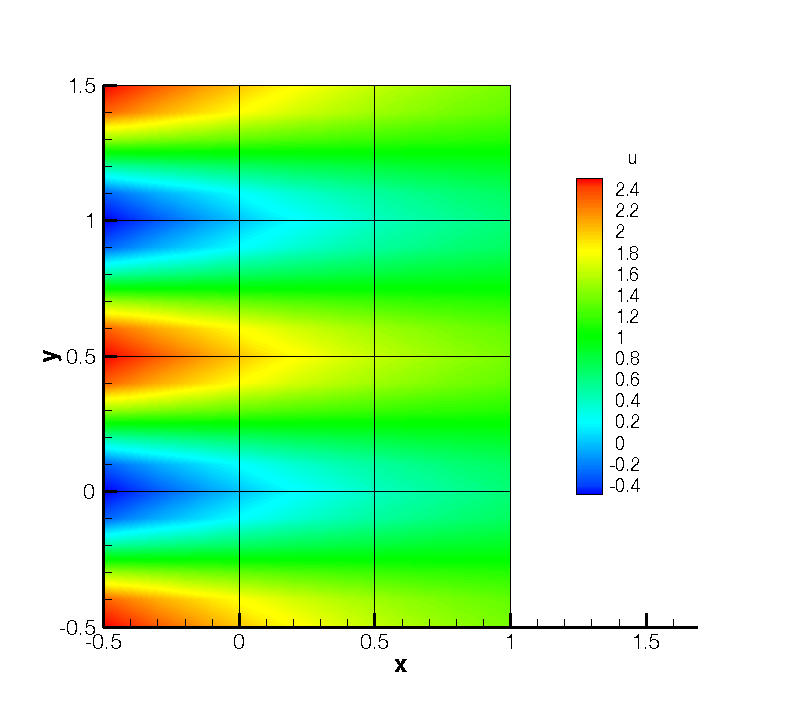
\includegraphics[width=7cm]{Figures/KF2DCVP8.png}
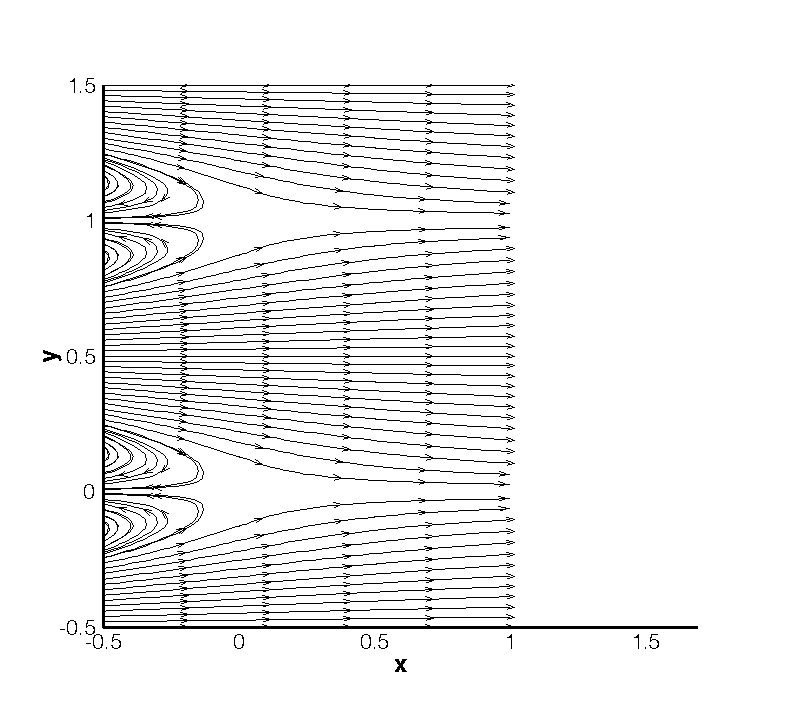
\includegraphics[width=7cm]{Figures/KF2DCVP8SL.png}
\caption{Velocity profiles for the Kovasznay Flow (2D).}
\end{center}
\end{figure}

\newpage

\subsubsection{2. Laminar Channel Flow 2D}
\label{LaminarChannelFlow2D}
The following example demonstrates the application of the \hyperref[IncNSsolver]{incompressible Navier-Stokes solver} using the \hyperref[VCSscheme]{Velocity Correction Scheme} algorithm for modelling 2D laminar channel flow. A skew-symmetric advection form has been used.

\textbf{Background}

The governing equation is the unsteady incompressible Navier-Stokes equation:
\begin{equation}
\begin{cases}
\frac{\partial \textbf{u}}{\partial t} + \textbf{u} \cdot \nabla \textbf{u} = - \nabla p + \nu \nabla^2 \textbf{u} + f \\
\nabla \cdot \textbf{u} = 0
\end{cases}
\end{equation}

In the following we will numerically solve for the two dimensional velocity and pressure field for steady boundary conditions. The Reynolds number under consideration is 1.

\textbf{Geometry}

The geometry under consideration is a 2D square channel with unit length and height (\textit{i.e.} $D=1$). The channel is modelled using 4 quadrilateral elements.

\textbf{Input parameters}

The session file can be found in the tests folder under the IncNavierStokesSolver folder and is named ChanFlow\_m3\_SKS.xml.

\paragraph{Expansion:~} In this example we will use a quadratic polynomial expansion (\textit{i.e.} $P=3$).
\begin{lstlisting}[style=XMLStyle]
<EXPANSIONS>
  <E COMPOSITE="C[0]" NUMMODES="3" FIELDS="u,v,p" TYPE="MODIFIED" />
</EXPANSIONS>
\end{lstlisting}

\paragraph{Solver information:~} Note the use of the Skew-symmetric option for the advection form.
\begin{lstlisting}[style=XMLStyle]
<SOLVERINFO>
  <I PROPERTY="EQTYPE" VALUE="UnsteadyNavierStokes" />
  <I PROPERTY="SolverType" VALUE="VelocityCorrectionScheme" />
  <I PROPERTY="EvolutionOperator" VALUE="SkewSymmetric" />
  <I PROPERTY="Projection" VALUE="Galerkin" />
  <I PROPERTY="TimeIntegrationMethod" VALUE="IMEXOrder1" />
</SOLVERINFO>
\end{lstlisting}

\paragraph{Parameters:~} Setting the mean inlet velocity to 1, allows us to define the kinematic viscosity as $\nu = \frac{UD}{Re}=1$.
\begin{lstlisting}[style=XMLStyle]
<PARAMETERS>
  <P> TimeStep = 0.001     </P>
  <P> NumSteps = 1000      </P>
  <P> IO_CheckSteps = 1000 </P>
  <P> IO_InfoSteps = 1000  </P>
  <P> Kinvis = 1           </P>
</PARAMETERS>
\end{lstlisting}

\paragraph{Boundary conditions:~} Boundary conditions have been defined on the walls and at the inflow (regions 0 and 1) as Dirichlet for the velocity field and as high-order for the pressure. At the outflow the velocity is left free using Neumann boundary conditions and the pressure is set to zero using Dirichlet.
\begin{lstlisting}[style=XMLStyle]
        <BOUNDARYCONDITIONS>
   			<REGION REF="0">
     			<D VAR="u" VALUE="0" />
     			<D VAR="v" VALUE="0" />
     			<N VAR="p" USERDEFINEDTYPE="H" VALUE="0" />
   			</REGION>
   			<REGION REF="1">
     			<D VAR="u" VALUE="y*(1-y)" />
     			<D VAR="v" VALUE="0" />
     			<N VAR="p" USERDEFINEDTYPE="H" VALUE="0" />
   			</REGION>
   			<REGION REF="2">
     			<N VAR="u" VALUE="0" />
     			<N VAR="v" VALUE="0" />
     			<D VAR="p" VALUE="0" />
   			</REGION>
		</BOUNDARYCONDITIONS>
\end{lstlisting}

\paragraph{Functions:~} Initial conditions are set to zero and the known exact solution, if provided, is used to calculate the error, which, for this case, is roughly the machine precision ($~10^{-15}$).
\begin{lstlisting}[style=XMLStyle]
		<FUNCTION NAME="InitialConditions">
  			<E VAR="u" VALUE="0" />
  			<E VAR="v" VALUE="0" />
  			<E VAR="p" VALUE="0" />
		</FUNCTION>
		<FUNCTION NAME="ExactSolution">
  			<E VAR="u" VALUE="y*(1-y)" />
  			<E VAR="v" VALUE="0" />
  			<E VAR="p" VALUE="-2*Kinvis*(x-1)" />
		</FUNCTION>
\end{lstlisting}

%\textbf{Usage}
%./IncNaverStokesSolver ChanFlow\_m3\_SKS.xml

\begin{figure}
\begin{center}
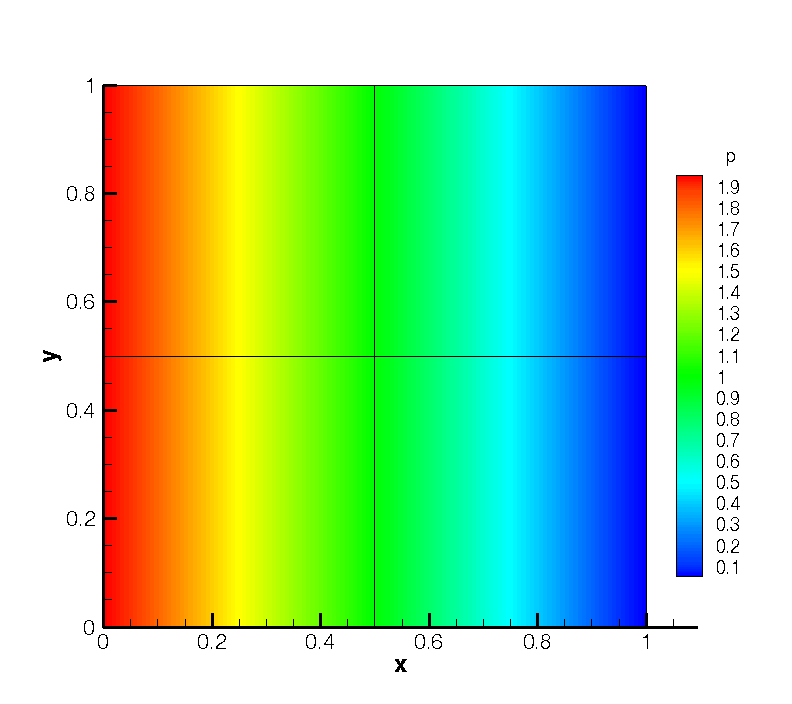
\includegraphics[width=7cm]{Figures/CF2DSKP3PR.png}
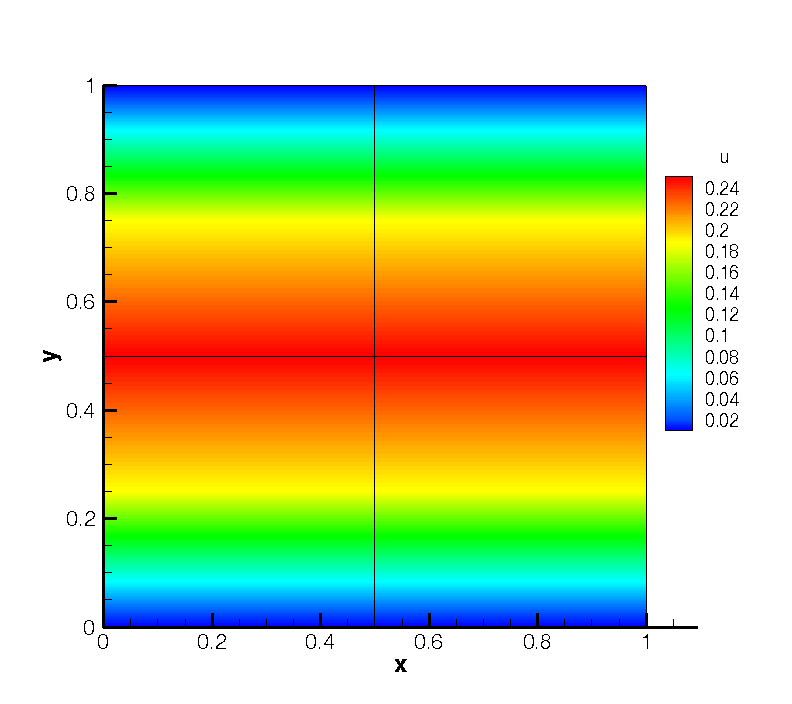
\includegraphics[width=7cm]{Figures/CF2DSKP3.png}
\caption{Pressure and velocity profiles for the laminar channel flow (2D).}
\end{center}
\end{figure}

\subsubsection{3. Laminar Channel Flow 3D}
The following example demonstrates the application of the \hyperref[IncNSsolver]{incompressible Navier-Stokes solver} using the \hyperref[VCSscheme]{Velocity Correction Scheme} algorithm for modelling 3D laminar channel flow.

\textbf{Background}

The governing equation is the unsteady incompressible Navier-Stokes equation:
\begin{equation}
\begin{cases}
\frac{\partial \textbf{u}}{\partial t} + \textbf{u} \cdot \nabla \textbf{u} = - \nabla p + \nu \nabla^2 \textbf{u} + f \\
\nabla \cdot \textbf{u} = 0
\end{cases}
\end{equation}

In the following we will numerically solve for the three dimensional velocity and pressure field for steady boundary conditions. The Reynolds number under consideration is 1.

\textbf{Geometry}

The geometry under consideration is a 3D square channel with unit length and height (\textit{i.e.} $D=1$). The channel is modelled using tetrahedral elements.

\textbf{Input parameters}

The session file can be found in the tests folder under the IncNavierStokesSolver folder and is named Tet\_channel\_m8\_par.xml.

\paragraph{Expansion:~} In this example we will use a 7th order polynomial expansion (\textit{i.e.} $P=8$).
\begin{lstlisting}[style=XMLStyle]
<EXPANSIONS>
  <E COMPOSITE="C[0]" NUMMODES="8" FIELDS="u,v,w,p" TYPE="MODIFIED" />
</EXPANSIONS>
\end{lstlisting}

\paragraph{Solver information:~} These information are given by
\begin{lstlisting}[style=XMLStyle]
<SOLVERINFO>
  <I PROPERTY="SolverType" VALUE="VelocityCorrectionScheme" />
  <I PROPERTY="EQTYPE" VALUE="UnsteadyNavierStokes" />
  <I PROPERTY="AdvectionForm" VALUE="Convective" />
  <I PROPERTY="Projection" VALUE="Galerkin" />
  <I PROPERTY="TimeIntegrationMethod" VALUE="IMEXOrder1" />
</SOLVERINFO>
\end{lstlisting}

\paragraph{Parameters:~} Setting the mean inlet velocity to 1, allows us to define the kinematic viscosity as $\nu = \frac{UD}{Re}=1$.
\begin{lstlisting}[style=XMLStyle]
<PARAMETERS>
  <P> TimeStep      = 0.001 </P>
  <P> NumSteps      = 10 </P>
  <P> IO_CheckSteps = 10    </P>
  <P> IO_InfoSteps  = 10    </P>
  <P> Kinvis        = 1   </P>
  <P> IterativeSolverTolerance = 1e-10 </P>
</PARAMETERS>
\end{lstlisting}

\paragraph{Boundary conditions:~} The boundary conditions are defined by
\begin{lstlisting}[style=XMLStyle]
        <BOUNDARYREGIONS>
            <B ID="0"> C[1] </B>    <!-- Inlet -->
            <B ID="1"> C[6] </B>    <!-- Outlet -->
            <B ID="2"> C[2] </B>    <!-- Wall -->
            <B ID="3"> C[3] </B>    <!-- Wall left -->
            <B ID="4"> C[4] </B>    <!-- Wall -->
            <B ID="5"> C[5] </B>    <!-- Wall right -->
        </BOUNDARYREGIONS>

        <BOUNDARYCONDITIONS>
            <REGION REF="0">
                <D VAR="u" VALUE="0" />
                <D VAR="v" VALUE="0" />
                <D VAR="w" VALUE="y*(1-y)" />
                <N VAR="p" USERDEFINEDTYPE="H" VALUE="0" />
            </REGION>
            <REGION REF="1">
                <N VAR="u" VALUE="0" />
                <N VAR="v" VALUE="0" />
                <N VAR="w" VALUE="0" />
                <D VAR="p" VALUE="0" />
            </REGION>
            <REGION REF="2">
                <D VAR="u" VALUE="0" />
                <D VAR="v" VALUE="0" />
                <D VAR="w" VALUE="0" />
                <N VAR="p" USERDEFINEDTYPE="H" VALUE="0" />
            </REGION>
            <REGION REF="3">
                <D VAR="u" VALUE="0" />
                <D VAR="v" VALUE="0" />
                <D VAR="w" VALUE="y*(1-y)" />
                <N VAR="p" USERDEFINEDTYPE="H" VALUE="0" />
            </REGION>
            <REGION REF="4">
                <D VAR="u" VALUE="0" />
                <D VAR="v" VALUE="0" />
                <D VAR="w" VALUE="0" />
                <N VAR="p" USERDEFINEDTYPE="H" VALUE="0" />
            </REGION>
            <REGION REF="5">
                <D VAR="u" VALUE="0" />
                <D VAR="v" VALUE="0" />
                <D VAR="w" VALUE="y*(1-y)" />
                <N VAR="p" USERDEFINEDTYPE="H" VALUE="0" />
            </REGION>
        </BOUNDARYCONDITIONS>
\end{lstlisting}

\paragraph{Functions:~} The exact solution is known in this case, and is therefore used to calculate the error.
\begin{lstlisting}[style=XMLStyle]
        <FUNCTION NAME="ExactSolution">
            <E VAR="u" VALUE="0" />
            <E VAR="v" VALUE="0" />
            <E VAR="w" VALUE="y*(1-y)" />
            <E VAR="p" VALUE="-2*Kinvis*(z-1)" />
        </FUNCTION>
        <FUNCTION NAME="InitialConditions">
            <E VAR="u" VALUE="0" />
            <E VAR="v" VALUE="0" />
            <E VAR="w" VALUE="y*(1-y)" />
            <E VAR="p" VALUE="-2*Kinvis*(z-1)" />
        </FUNCTION>
\end{lstlisting}

%\textbf{Usage}
%./IncNaverStokesSolver Tet\_channel\_m8\_par.xml

\begin{figure}
\begin{center}
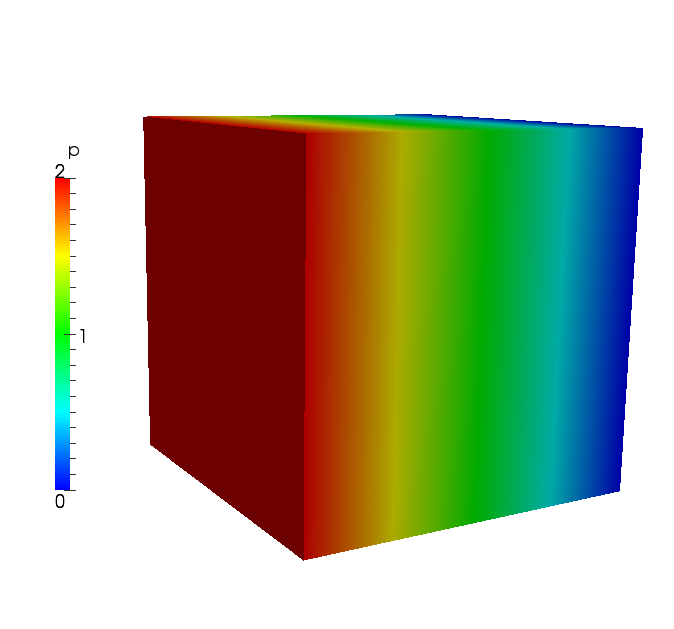
\includegraphics[width=7cm]{Figures/CF3DP8PR.png}
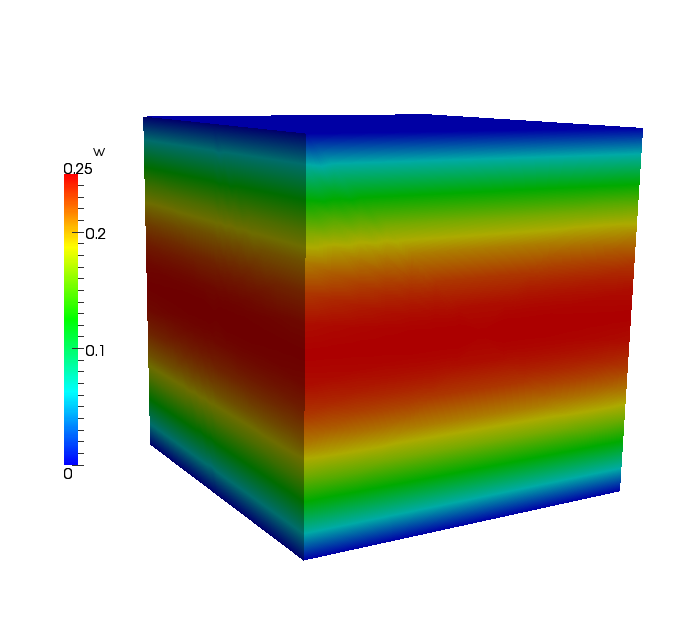
\includegraphics[width=7cm]{Figures/CF3DP8.png}
\caption{Pressure and velocity profiles for the laminar channel flow (full 3D).}
\end{center}
\end{figure}


\subsubsection{4. Laminar Channel Flow Quasi-3D}
In this example we reuse the 2D mesh used before for the \hyperref[LaminarChannelFlow2D]{2D Laminar Channel Flow} example, and we add mathematically the third dimension assuming an expansion along z with a Fourier series. The example is an application of the \hyperref[IncNSsolver]{incompressible Navier-Stokes solver} using the \hyperref[VCSscheme]{Velocity Correction Scheme} algorithm.

\textbf{Background}

The governing equation is the unsteady incompressible Navier-Stokes equation:
\begin{equation}
\begin{cases}
\frac{\partial \textbf{u}}{\partial t} + \textbf{u} \cdot \nabla \textbf{u} = - \nabla p + \nu \nabla^2 \textbf{u} + f \\
\nabla \cdot \textbf{u} = 0
\end{cases}
\end{equation}

The Reynolds number under consideration is 1.

\textbf{Geometry}

The geometry under consideration is a 2D square channel with unit length and height (\textit{i.e.} $D=1$). The channel is modelled using 4 quadrilateral elements. The geometry as well as the mesh is identical to that used in the \hyperref[LaminarChannelFlow2D]{2D Laminar Channel Flow} example.

\textbf{Input parameters}

\paragraph{Expansion:~} In this example we will use a quadratic polynomial expansion (\textit{i.e.} $P=3$).
\begin{lstlisting}[style=XMLStyle]
<EXPANSIONS>
  <E COMPOSITE="C[0]" NUMMODES="3" FIELDS="u,v,w,p" TYPE="MODIFIED" />
</EXPANSIONS>
\end{lstlisting}

\paragraph{Solver information:~}  The flag 
\begin{lstlisting}[style=XMLStyle] 
<I PROPERTY="HOMOGENEOUS" VALUE="1D"/> 
\end{lstlisting} 
is informing the code that, even if the mesh is 2D, the problem is 3D and the third direction needs to be added with a Fourier series. An extra flag could be added to activate the FFT routines inside the code 
\begin{lstlisting}[style=XMLStyle]
<I PROPERTY="USEFFT" VALUE="FFTW"/>
\end{lstlisting} 

In this case Nektar++ uses the FFTW library to move the degrees of freedom from wave to real space. HomModesZ and LZ set the number of Fourier modes and the length of the third direction respectively.
\begin{lstlisting}[style=XMLStyle]
  <SOLVERINFO>
    <I PROPERTY="EQTYPE" VALUE="UnsteadyNavierStokes"/>
    <I PROPERTY="SolverType"  VALUE="VelocityCorrectionScheme"/>
    <I PROPERTY="EvolutionOperator" VALUE="Nonlinear" />
    <I PROPERTY="Projection" VALUE="Galerkin"/>
    <I PROPERTY="TimeIntegrationMethod" VALUE="IMEXOrder3"/>
    <I PROPERTY="HOMOGENEOUS" VALUE="1D"/>
  </SOLVERINFO>
\end{lstlisting}

\paragraph{Parameters:~} Setting the mean inlet velocity to 1, allows us to define the kinematic viscosity as $\nu = \frac{UD}{Re}=1$.
\begin{lstlisting}[style=XMLStyle]
  <PARAMETERS>
    <P> TimeStep      = 0.001    </P>
    <P> NumSteps      = 1000     </P>
    <P> IO_CheckSteps = 1000     </P>
    <P> IO_InfoSteps  = 1000     </P>
    <P> Kinvis        = 1        </P>
    <P> HomModesZ     = 20       </P>
    <P> LZ            = 1.0      </P>
  </PARAMETERS>
\end{lstlisting}

\paragraph{Boundary conditions:~} Boundary conditions have been defined on the walls and at the inflow (regions 0 and 1) as Dirichlet for the velocity field and as high-order for the pressure. At the outflow the velocity is left free using Neumann boundary conditions and the pressure is set to zero using Dirichlet.
\begin{lstlisting}[style=XMLStyle]
  <BOUNDARYCONDITIONS>
    <REGION REF="0">
      <D VAR="u" VALUE="0" />
      <D VAR="v" VALUE="0" />
      <D VAR="w" VALUE="0" />
      <N VAR="p" USERDEFINEDTYPE="H" VALUE="0" />
    </REGION>
    <REGION REF="1">
      <D VAR="u" VALUE="y*(1-y)" />
      <D VAR="v" VALUE="0" />
      <D VAR="w" VALUE="0" />
      <N VAR="p" USERDEFINEDTYPE="H" VALUE="0" />
    </REGION>
    <REGION REF="2">
      <N VAR="u" VALUE="0" />
      <N VAR="v" VALUE="0" />
      <N VAR="w" VALUE="0" />
      <D VAR="p" VALUE="0" />
    </REGION>
  </BOUNDARYCONDITIONS>
\end{lstlisting}

\paragraph{Functions:~} Homogeneous initial conditions are imposed and an analytical formulation of the exact solution is provided.
\begin{lstlisting}[style=XMLStyle]
  <FUNCTION NAME="InitialConditions">
     <E VAR="u" VALUE="0" />
     <E VAR="v" VALUE="0" />
     <E VAR="w" VALUE="0" />
     <E VAR="p" VALUE="0" />
  </FUNCTION>

  <FUNCTION NAME="ExactSolution">
     <E VAR="u" VALUE="y*(1-y)" />
     <E VAR="v" VALUE="0" />
     <E VAR="w" VALUE="0" />
     <E VAR="p" VALUE="-2*Kinvis*(x-1)" />
  </FUNCTION>
\end{lstlisting}

%\textbf{Usage}
%./IncNaverStokesSolver session.xml

\begin{figure}
\begin{center}
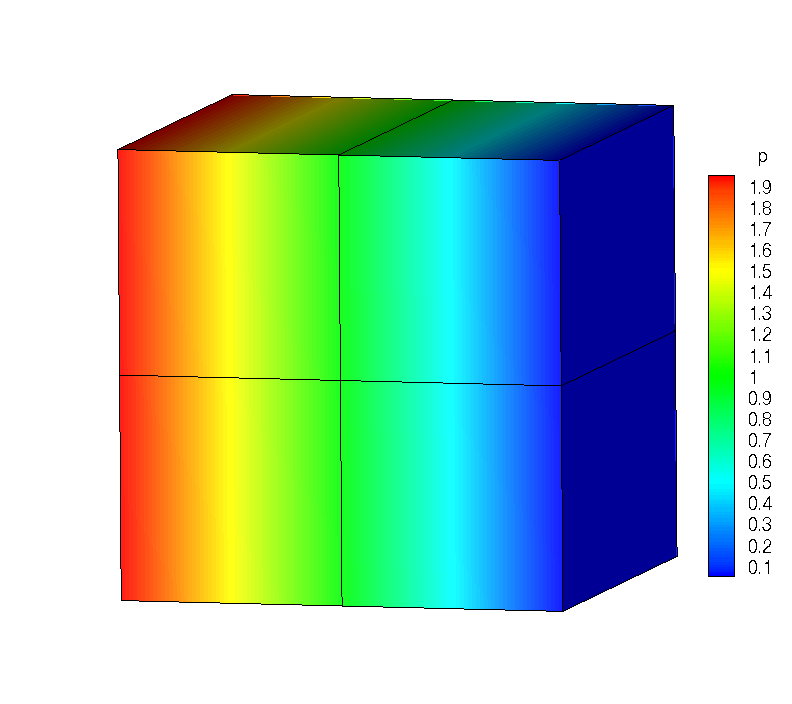
\includegraphics[width=7cm]{Figures/CF3DCVP3PR.png}
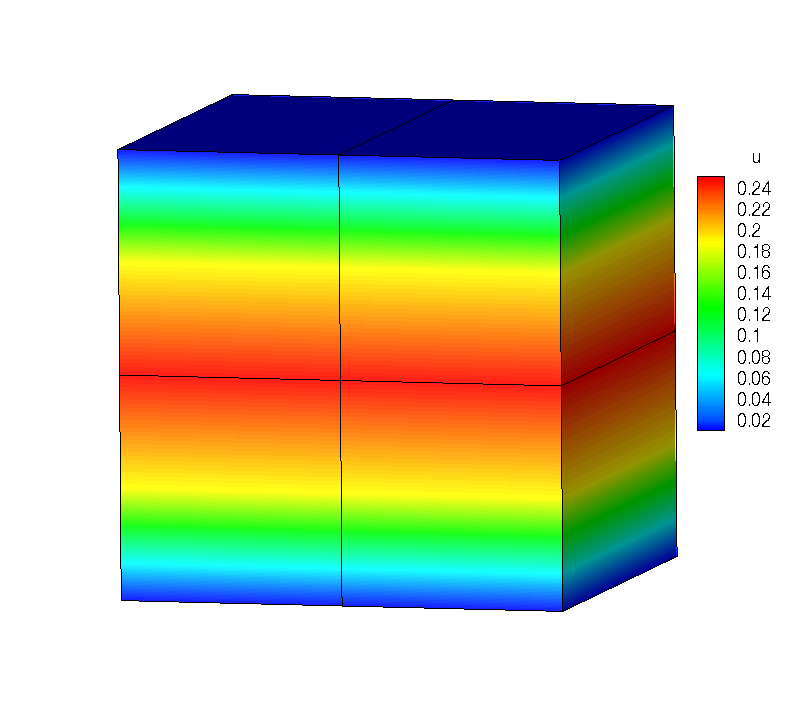
\includegraphics[width=7cm]{Figures/CF3DCVP3.png}
\caption{Pressure and velocity profiles for the laminar channel flow (quasi 3D).}
\end{center}
\end{figure}


\subsubsection{5. Turbulent Channel Flow Quasi-3D}
In this example we use a 2D mesh for channel flow, and we add mathematically the third dimension assuming an expansion along z with a Fourier series. The example is an application of the \hyperref[IncNSsolver]{incompressible Navier-Stokes solver} using the \hyperref[VCSscheme]{Velocity Correction Scheme} algorithm in order to solve for turbulent channel flow.

\textbf{Background}

The governing equation is the unsteady incompressible Navier-Stokes equation:
\begin{equation}
\begin{cases}
\frac{\partial \textbf{u}}{\partial t} + \textbf{u} \cdot \nabla \textbf{u} = - \nabla p + \nu \nabla^2 \textbf{u} + f \\
\nabla \cdot \textbf{u} = 0
\label{IncNS_equations}
\end{cases}
\end{equation}

The Reynolds number under consideration is 2000.

\textbf{Geometry}

The geometry under consideration is a 2D square channel with height of 2 units (\textit{i.e.} $D=2$), and length of 12.57. The channel is modelled using quadrilateral elements.
\begin{figure}
\begin{center}
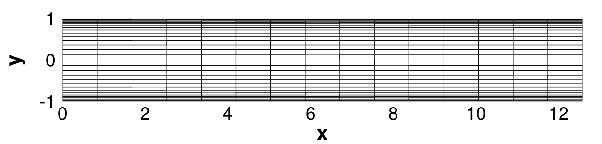
\includegraphics[width=10cm]{Figures/ChanMesh.png}
\caption{Mesh used for the turbulent channel flow (quasi-3D).}
\end{center}
\end{figure}

\textbf{Input parameters}

For this tutorial, the input file (in the \hyperref[XMLformat]{\nekpp input format}) used can be found in Nektar++/solvers/IncNavierStokesSolver/Examples/TurbChFl\_3DH1D.xml.

\paragraph{Expansion:~} In this example we will use a quadratic polynomial expansion (\textit{i.e.} $P=3$).
\begin{lstlisting}[style=XMLStyle]
<EXPANSIONS>
  <E COMPOSITE="C[0]" NUMMODES="3" FIELDS="u,v,w,p" TYPE="MODIFIED" />
</EXPANSIONS>
\end{lstlisting}

\paragraph{Solver information:~} The flag 
\begin{lstlisting}[style=XMLStyle]
<I PROPERTY="HOMOGENEOUS" VALUE="1D"/>
\end{lstlisting}
is informing the code that, even if the mesh is 2D, the problem is 3D and the third direction needs to be added with a Fourier series. An extra flag could be added to activate the FFT routines inside the code 
\begin{lstlisting}[style=XMLStyle]
<I PROPERTY="USEFFT" VALUE="FFTW"/>
\end{lstlisting}
In this case Nektar++ uses the FFTW library to move the degrees of freedom from wave to real space. HomModesZ and LZ set the number of Fourier modes and the length of the third direction respectively.

\begin{lstlisting}[style=XMLStyle]
    <SOLVERINFO>
      <I PROPERTY="SolverType"  VALUE="VelocityCorrectionScheme"/>
      <I PROPERTY="EQTYPE" VALUE="UnsteadyNavierStokes"/>
      <I PROPERTY="AdvectionForm" VALUE="Convective"/>
      <I PROPERTY="Projection" VALUE="Galerkin"/>
      <I PROPERTY="TimeIntegrationMethod" VALUE="IMEXOrder2"/>
      <I PROPERTY="HOMOGENEOUS" VALUE="1D"/>
    </SOLVERINFO>
\end{lstlisting}

\paragraph{Parameters:~} Setting the mean inlet velocity to 1, allows us to define the kinematic viscosity as $\nu = \frac{UD}{Re}=1$.
\begin{lstlisting}[style=XMLStyle]
    <PARAMETERS>
      <P> TimeStep      = 0.0001      </P>
      <P> NumSteps      = 10000       </P>
      <P> IO_CheckSteps = 1000       </P>
      <P> IO_InfoSteps  = 10       </P>
      <P> Re            = 2000       </P>
      <P> Kinvis        = 1.0/Re     </P>
      <P> HomModesZ     = 32          </P>
      <P> LZ            = 4*PI/3     </P>
    </PARAMETERS>
\end{lstlisting}

\paragraph{Boundary conditions:~} The boundary conditions are defined by
\begin{lstlisting}[style=XMLStyle]
    <BOUNDARYREGIONS>
      <B ID="0"> C[1] </B> //walls
      <B ID="1"> C[2] </B> //inflow
      <B ID="2"> C[3] </B> //outflow
    </BOUNDARYREGIONS>

    <BOUNDARYCONDITIONS>
      <REGION REF="0">
        <D VAR="u" VALUE="0" />
        <D VAR="v" VALUE="0" />
        <D VAR="w" VALUE="0" />
        <N VAR="p" USERDEFINEDTYPE="H" VALUE="0" />  
      </REGION>
      <REGION REF="1">
        <P VAR="u" VALUE="[2]" />
        <P VAR="v" VALUE="[2]" />
        <P VAR="w" VALUE="[2]" />
        <P VAR="p" VALUE="[2]" />
      </REGION>
      <REGION REF="2">
        <P VAR="u" VALUE="[1]" />
        <P VAR="v" VALUE="[1]" />
        <P VAR="w" VALUE="[1]" />
        <P VAR="p" VALUE="[1]" />
      </REGION>
    </BOUNDARYCONDITIONS>
\end{lstlisting}

\paragraph{Functions:~} The initial conditions and the body force (\textit{i.e.} $f$ in the governing equations \ref{IncNS_equations}) are given by
\begin{lstlisting}[style=XMLStyle]
   <FUNCTION NAME="InitialConditions">
     <E VAR="u" VALUE="1" />
     <E VAR="v" VALUE="0" />
     <E VAR="w" VALUE="0" />
     <E VAR="p" VALUE="0" />
   </FUNCTION>
   
   <FUNCTION NAME="BodyForce">
          <E VAR="u" VALUE="2*Kinvis" />
          <E VAR="v" VALUE="0" />
          <E VAR="w" VALUE="0" />
   </FUNCTION>
\end{lstlisting}

%\textbf{Usage} 
%./IncNaverStokesSolver TurbChFl\_3DH1D.xml 

\begin{figure}
\begin{center}
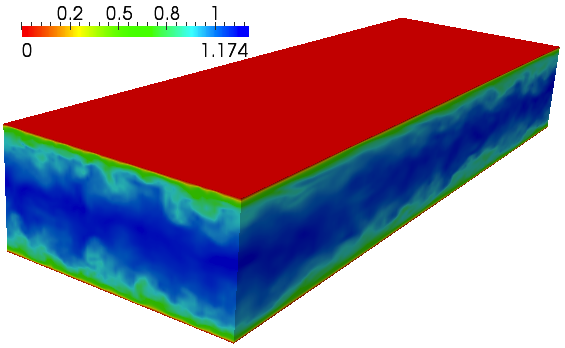
\includegraphics[width=12cm]{Figures/ChanCont.png}
\caption{Velocity profile of the turbulent channel flow (quasi-3D).}
\end{center}
\end{figure}


\subsubsection{6. Laminar Channel Flow 3D}
The following example demonstrates the application of the \hyperref[IncNSsolver]{incompressible Navier-Stokes solver} using the \hyperref[VCSscheme]{Velocity Correction Scheme} algorithm for modelling 3D laminar channel flow.

\textbf{Background}

The governing equation is the unsteady incompressible Navier-Stokes equation:
\begin{equation}
\begin{cases}
\frac{\partial \textbf{u}}{\partial t} + \textbf{u} \cdot \nabla \textbf{u} = - \nabla p + \nu \nabla^2 \textbf{u} + f \\
\nabla \cdot \textbf{u} = 0
\end{cases}
\end{equation}

In the following we will numerically solve for the three dimensional velocity and pressure field for steady boundary conditions. The Reynolds number under consideration is 1.

\textbf{Geometry}

The geometry under consideration is a 3D square channel with unit length and height (\textit{i.e.} $D=1$). The channel is modelled using tetrahedral elements.

\textbf{Input parameters}

The session file can be found in the tests folder under the IncNavierStokesSolver folder and is named Tet\_channel\_m8\_par.xml.

\paragraph{Expansion:~} In this example we will use a 7th order polynomial expansion (\textit{i.e.} $P=8$).
\begin{lstlisting}[style=XMLStyle]
<EXPANSIONS>
  <E COMPOSITE="C[0]" NUMMODES="8" FIELDS="u,v,w,p" TYPE="MODIFIED" />
</EXPANSIONS>
\end{lstlisting}

\paragraph{Solver information:~} These information are given by
\begin{lstlisting}[style=XMLStyle]
<SOLVERINFO>
  <I PROPERTY="SolverType" VALUE="VelocityCorrectionScheme" />
  <I PROPERTY="EQTYPE" VALUE="UnsteadyNavierStokes" />
  <I PROPERTY="AdvectionForm" VALUE="Convective" />
  <I PROPERTY="Projection" VALUE="Galerkin" />
  <I PROPERTY="TimeIntegrationMethod" VALUE="IMEXOrder1" />
</SOLVERINFO>
\end{lstlisting}

\paragraph{Parameters:~} Setting the mean inlet velocity to 1, allows us to define the kinematic viscosity as $\nu = \frac{UD}{Re}=1$.
\begin{lstlisting}[style=XMLStyle]
<PARAMETERS>
  <P> TimeStep      = 0.001 </P>
  <P> NumSteps      = 10 </P>
  <P> IO_CheckSteps = 10    </P>
  <P> IO_InfoSteps  = 10    </P>
  <P> Kinvis        = 1   </P>
  <P> IterativeSolverTolerance = 1e-10 </P>
</PARAMETERS>
\end{lstlisting}

\paragraph{Boundary conditions:~} The boundary conditions are defined by
\begin{lstlisting}[style=XMLStyle]
        <BOUNDARYREGIONS>
            <B ID="0"> C[1] </B>    <!-- Inlet -->
            <B ID="1"> C[6] </B>    <!-- Outlet -->
            <B ID="2"> C[2] </B>    <!-- Wall -->
            <B ID="3"> C[3] </B>    <!-- Wall left -->
            <B ID="4"> C[4] </B>    <!-- Wall -->
            <B ID="5"> C[5] </B>    <!-- Wall right -->
        </BOUNDARYREGIONS>

        <BOUNDARYCONDITIONS>
            <REGION REF="0">
                <D VAR="u" VALUE="0" />
                <D VAR="v" VALUE="0" />
                <D VAR="w" VALUE="y*(1-y)" />
                <N VAR="p" USERDEFINEDTYPE="H" VALUE="0" />
            </REGION>
            <REGION REF="1">
                <N VAR="u" VALUE="0" />
                <N VAR="v" VALUE="0" />
                <N VAR="w" VALUE="0" />
                <D VAR="p" VALUE="0" />
            </REGION>
            <REGION REF="2">
                <D VAR="u" VALUE="0" />
                <D VAR="v" VALUE="0" />
                <D VAR="w" VALUE="0" />
                <N VAR="p" USERDEFINEDTYPE="H" VALUE="0" />
            </REGION>
            <REGION REF="3">
                <D VAR="u" VALUE="0" />
                <D VAR="v" VALUE="0" />
                <D VAR="w" VALUE="y*(1-y)" />
                <N VAR="p" USERDEFINEDTYPE="H" VALUE="0" />
            </REGION>
            <REGION REF="4">
                <D VAR="u" VALUE="0" />
                <D VAR="v" VALUE="0" />
                <D VAR="w" VALUE="0" />
                <N VAR="p" USERDEFINEDTYPE="H" VALUE="0" />
            </REGION>
            <REGION REF="5">
                <D VAR="u" VALUE="0" />
                <D VAR="v" VALUE="0" />
                <D VAR="w" VALUE="y*(1-y)" />
                <N VAR="p" USERDEFINEDTYPE="H" VALUE="0" />
            </REGION>
        </BOUNDARYCONDITIONS>
\end{lstlisting}

\paragraph{Functions:~} The exact solution is known in this case, and is therefore used to calculate the error.
\begin{lstlisting}[style=XMLStyle]
        <FUNCTION NAME="ExactSolution">
            <E VAR="u" VALUE="0" />
            <E VAR="v" VALUE="0" />
            <E VAR="w" VALUE="y*(1-y)" />
            <E VAR="p" VALUE="-2*Kinvis*(z-1)" />
        </FUNCTION>
        <FUNCTION NAME="InitialConditions">
            <E VAR="u" VALUE="0" />
            <E VAR="v" VALUE="0" />
            <E VAR="w" VALUE="y*(1-y)" />
            <E VAR="p" VALUE="-2*Kinvis*(z-1)" />
        </FUNCTION>
\end{lstlisting}

%\textbf{Usage}
%./IncNaverStokesSolver Tet\_channel\_m8\_par.xml

\begin{figure}
\begin{center}
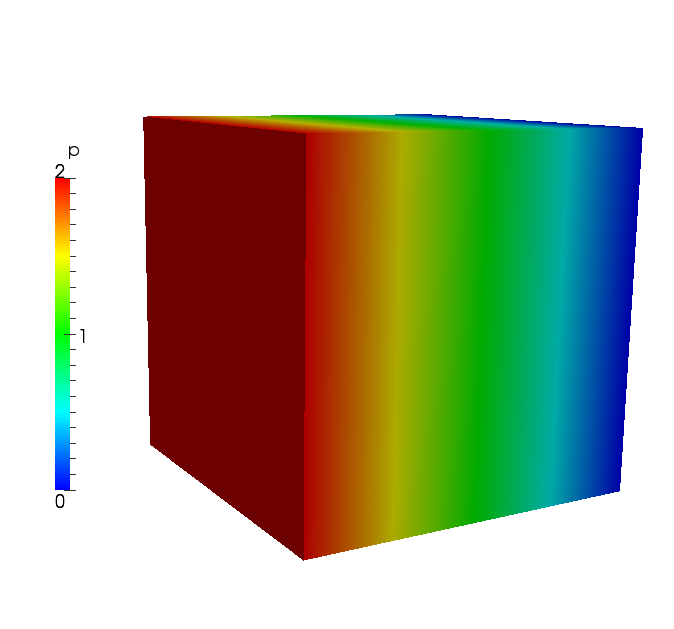
\includegraphics[width=7cm]{Figures/CF3DP8PR.png}
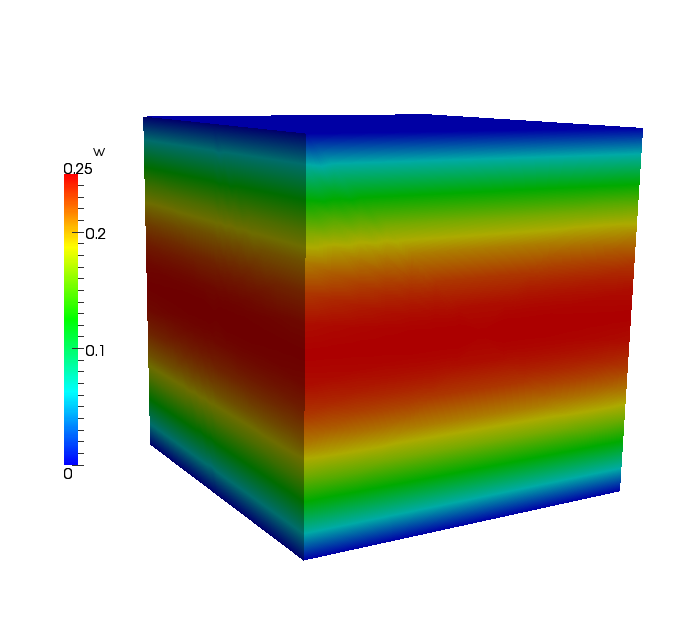
\includegraphics[width=7cm]{Figures/CF3DP8.png}
\caption{Pressure and velocity profiles for the laminar channel flow (full 3D).}
\end{center}
\end{figure}


\subsubsection{7. Laminar Channel Flow Quasi-3D}
In this example we reuse the 2D mesh used before for the \hyperref[LaminarChannelFlow2D]{2D Laminar Channel Flow} example, and we add mathematically the third dimension assuming an expansion along z with a Fourier series. The example is an application of the \hyperref[IncNSsolver]{incompressible Navier-Stokes solver} using the \hyperref[VCSscheme]{Velocity Correction Scheme} algorithm.

\textbf{Background}

The governing equation is the unsteady incompressible Navier-Stokes equation:
\begin{equation}
\begin{cases}
\frac{\partial \textbf{u}}{\partial t} + \textbf{u} \cdot \nabla \textbf{u} = - \nabla p + \nu \nabla^2 \textbf{u} + f \\
\nabla \cdot \textbf{u} = 0
\end{cases}
\end{equation}

The Reynolds number under consideration is 1.

\textbf{Geometry}

The geometry under consideration is a 2D square channel with unit length and height (\textit{i.e.} $D=1$). The channel is modelled using 4 quadrilateral elements. The geometry as well as the mesh is identical to that used in the \hyperref[LaminarChannelFlow2D]{2D Laminar Channel Flow} example.

\textbf{Input parameters}

\paragraph{Expansion:~} In this example we will use a quadratic polynomial expansion (\textit{i.e.} $P=3$).
\begin{lstlisting}[style=XMLStyle]
<EXPANSIONS>
  <E COMPOSITE="C[0]" NUMMODES="3" FIELDS="u,v,w,p" TYPE="MODIFIED" />
</EXPANSIONS>
\end{lstlisting}

\paragraph{Solver information:~}  The flag 
\begin{lstlisting}[style=XMLStyle] 
<I PROPERTY="HOMOGENEOUS" VALUE="1D"/> 
\end{lstlisting} 
is informing the code that, even if the mesh is 2D, the problem is 3D and the third direction needs to be added with a Fourier series. An extra flag could be added to activate the FFT routines inside the code 
\begin{lstlisting}[style=XMLStyle]
<I PROPERTY="USEFFT" VALUE="FFTW"/>
\end{lstlisting} 

In this case Nektar++ uses the FFTW library to move the degrees of freedom from wave to real space. HomModesZ and LZ set the number of Fourier modes and the length of the third direction respectively.
\begin{lstlisting}[style=XMLStyle]
  <SOLVERINFO>
    <I PROPERTY="EQTYPE" VALUE="UnsteadyNavierStokes"/>
    <I PROPERTY="SolverType"  VALUE="VelocityCorrectionScheme"/>
    <I PROPERTY="EvolutionOperator" VALUE="Nonlinear" />
    <I PROPERTY="Projection" VALUE="Galerkin"/>
    <I PROPERTY="TimeIntegrationMethod" VALUE="IMEXOrder3"/>
    <I PROPERTY="HOMOGENEOUS" VALUE="1D"/>
  </SOLVERINFO>
\end{lstlisting}

\paragraph{Parameters:~} Setting the mean inlet velocity to 1, allows us to define the kinematic viscosity as $\nu = \frac{UD}{Re}=1$.
\begin{lstlisting}[style=XMLStyle]
  <PARAMETERS>
    <P> TimeStep      = 0.001    </P>
    <P> NumSteps      = 1000     </P>
    <P> IO_CheckSteps = 1000     </P>
    <P> IO_InfoSteps  = 1000     </P>
    <P> Kinvis        = 1        </P>
    <P> HomModesZ     = 20       </P>
    <P> LZ            = 1.0      </P>
  </PARAMETERS>
\end{lstlisting}

\paragraph{Boundary conditions:~} Boundary conditions have been defined on the walls and at the inflow (regions 0 and 1) as Dirichlet for the velocity field and as high-order for the pressure. At the outflow the velocity is left free using Neumann boundary conditions and the pressure is set to zero using Dirichlet.
\begin{lstlisting}[style=XMLStyle]
  <BOUNDARYCONDITIONS>
    <REGION REF="0">
      <D VAR="u" VALUE="0" />
      <D VAR="v" VALUE="0" />
      <D VAR="w" VALUE="0" />
      <N VAR="p" USERDEFINEDTYPE="H" VALUE="0" />
    </REGION>
    <REGION REF="1">
      <D VAR="u" VALUE="y*(1-y)" />
      <D VAR="v" VALUE="0" />
      <D VAR="w" VALUE="0" />
      <N VAR="p" USERDEFINEDTYPE="H" VALUE="0" />
    </REGION>
    <REGION REF="2">
      <N VAR="u" VALUE="0" />
      <N VAR="v" VALUE="0" />
      <N VAR="w" VALUE="0" />
      <D VAR="p" VALUE="0" />
    </REGION>
  </BOUNDARYCONDITIONS>
\end{lstlisting}

\paragraph{Functions:~} Homogeneous initial conditions are imposed and an analytical formulation of the exact solution is provided.
\begin{lstlisting}[style=XMLStyle]
  <FUNCTION NAME="InitialConditions">
     <E VAR="u" VALUE="0" />
     <E VAR="v" VALUE="0" />
     <E VAR="w" VALUE="0" />
     <E VAR="p" VALUE="0" />
  </FUNCTION>

  <FUNCTION NAME="ExactSolution">
     <E VAR="u" VALUE="y*(1-y)" />
     <E VAR="v" VALUE="0" />
     <E VAR="w" VALUE="0" />
     <E VAR="p" VALUE="-2*Kinvis*(x-1)" />
  </FUNCTION>
\end{lstlisting}

%\textbf{Usage}
%./IncNaverStokesSolver session.xml

\begin{figure}
\begin{center}
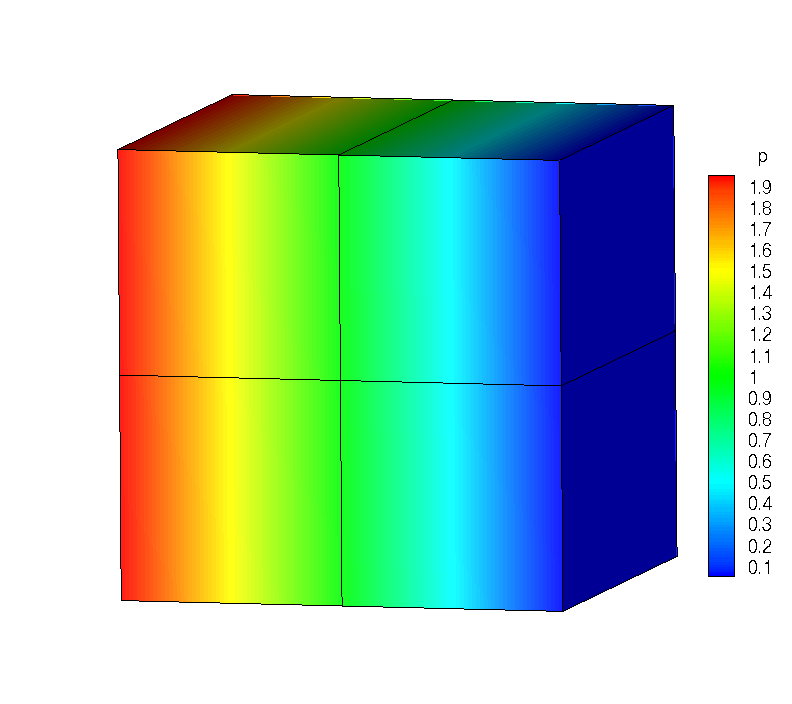
\includegraphics[width=7cm]{Figures/CF3DCVP3PR.png}
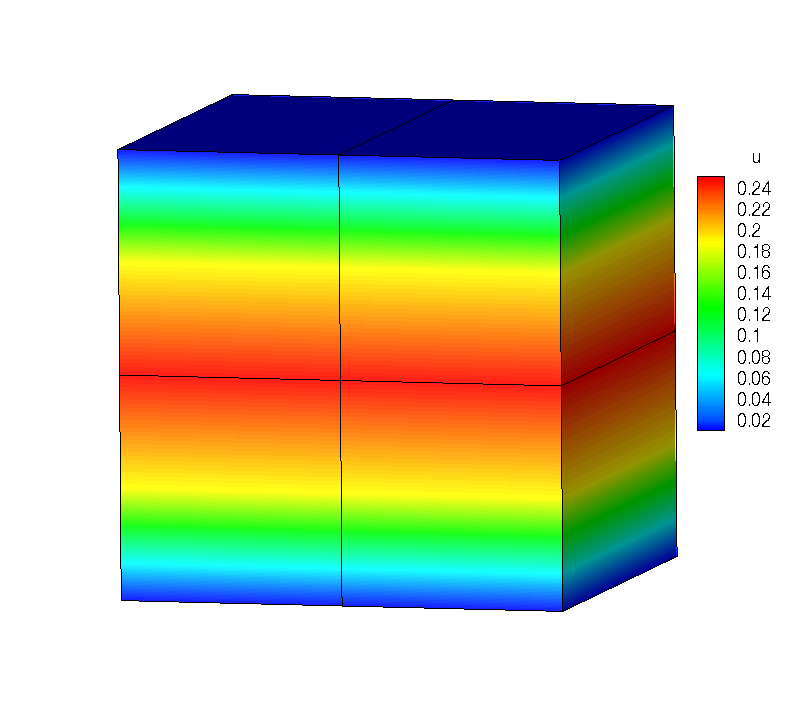
\includegraphics[width=7cm]{Figures/CF3DCVP3.png}
\caption{Pressure and velocity profiles for the laminar channel flow (quasi 3D).}
\end{center}
\end{figure}

\newpage


3.4/UserGuide/Examples/IncNavierStokesSolver/SteadyOseenFlow2D
3.4/UserGuide/Examples/IncNavierStokesSolver/Transient


\subsubsection{8. Turbulent Channel Flow Quasi-3D}
In this example we use a 2D mesh for channel flow, and we add mathematically the third dimension assuming an expansion along z with a Fourier series. The example is an application of the \hyperref[IncNSsolver]{incompressible Navier-Stokes solver} using the \hyperref[VCSscheme]{Velocity Correction Scheme} algorithm in order to solve for turbulent channel flow.

\textbf{Background}

The governing equation is the unsteady incompressible Navier-Stokes equation:
\begin{equation}
\begin{cases}
\frac{\partial \textbf{u}}{\partial t} + \textbf{u} \cdot \nabla \textbf{u} = - \nabla p + \nu \nabla^2 \textbf{u} + f \\
\nabla \cdot \textbf{u} = 0
\label{IncNS_equations}
\end{cases}
\end{equation}

The Reynolds number under consideration is 2000.

\textbf{Geometry}

The geometry under consideration is a 2D square channel with height of 2 units (\textit{i.e.} $D=2$), and length of 12.57. The channel is modelled using quadrilateral elements.
\begin{figure}
\begin{center}
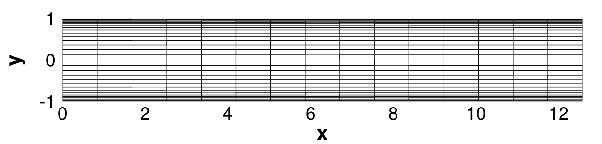
\includegraphics[width=10cm]{Figures/ChanMesh.png}
\caption{Mesh used for the turbulent channel flow (quasi-3D).}
\end{center}
\end{figure}

\textbf{Input parameters}

For this tutorial, the input file (in the \hyperref[XMLformat]{\nekpp input format}) used can be found in Nektar++/solvers/IncNavierStokesSolver/Examples/TurbChFl\_3DH1D.xml.

\paragraph{Expansion:~} In this example we will use a quadratic polynomial expansion (\textit{i.e.} $P=3$).
\begin{lstlisting}[style=XMLStyle]
<EXPANSIONS>
  <E COMPOSITE="C[0]" NUMMODES="3" FIELDS="u,v,w,p" TYPE="MODIFIED" />
</EXPANSIONS>
\end{lstlisting}

\paragraph{Solver information:~} The flag 
\begin{lstlisting}[style=XMLStyle]
<I PROPERTY="HOMOGENEOUS" VALUE="1D"/>
\end{lstlisting}
is informing the code that, even if the mesh is 2D, the problem is 3D and the third direction needs to be added with a Fourier series. An extra flag could be added to activate the FFT routines inside the code 
\begin{lstlisting}[style=XMLStyle]
<I PROPERTY="USEFFT" VALUE="FFTW"/>
\end{lstlisting}
In this case Nektar++ uses the FFTW library to move the degrees of freedom from wave to real space. HomModesZ and LZ set the number of Fourier modes and the length of the third direction respectively.

\begin{lstlisting}[style=XMLStyle]
    <SOLVERINFO>
      <I PROPERTY="SolverType"  VALUE="VelocityCorrectionScheme"/>
      <I PROPERTY="EQTYPE" VALUE="UnsteadyNavierStokes"/>
      <I PROPERTY="AdvectionForm" VALUE="Convective"/>
      <I PROPERTY="Projection" VALUE="Galerkin"/>
      <I PROPERTY="TimeIntegrationMethod" VALUE="IMEXOrder2"/>
      <I PROPERTY="HOMOGENEOUS" VALUE="1D"/>
    </SOLVERINFO>
\end{lstlisting}

\paragraph{Parameters:~} Setting the mean inlet velocity to 1, allows us to define the kinematic viscosity as $\nu = \frac{UD}{Re}=1$.
\begin{lstlisting}[style=XMLStyle]
    <PARAMETERS>
      <P> TimeStep      = 0.0001      </P>
      <P> NumSteps      = 10000       </P>
      <P> IO_CheckSteps = 1000       </P>
      <P> IO_InfoSteps  = 10       </P>
      <P> Re            = 2000       </P>
      <P> Kinvis        = 1.0/Re     </P>
      <P> HomModesZ     = 32          </P>
      <P> LZ            = 4*PI/3     </P>
    </PARAMETERS>
\end{lstlisting}

\paragraph{Boundary conditions:~} The boundary conditions are defined by
\begin{lstlisting}[style=XMLStyle]
    <BOUNDARYREGIONS>
      <B ID="0"> C[1] </B> //walls
      <B ID="1"> C[2] </B> //inflow
      <B ID="2"> C[3] </B> //outflow
    </BOUNDARYREGIONS>

    <BOUNDARYCONDITIONS>
      <REGION REF="0">
        <D VAR="u" VALUE="0" />
        <D VAR="v" VALUE="0" />
        <D VAR="w" VALUE="0" />
        <N VAR="p" USERDEFINEDTYPE="H" VALUE="0" />  
      </REGION>
      <REGION REF="1">
        <P VAR="u" VALUE="[2]" />
        <P VAR="v" VALUE="[2]" />
        <P VAR="w" VALUE="[2]" />
        <P VAR="p" VALUE="[2]" />
      </REGION>
      <REGION REF="2">
        <P VAR="u" VALUE="[1]" />
        <P VAR="v" VALUE="[1]" />
        <P VAR="w" VALUE="[1]" />
        <P VAR="p" VALUE="[1]" />
      </REGION>
    </BOUNDARYCONDITIONS>
\end{lstlisting}

\paragraph{Functions:~} The initial conditions and the body force (\textit{i.e.} $f$ in the governing equations \ref{IncNS_equations}) are given by
\begin{lstlisting}[style=XMLStyle]
   <FUNCTION NAME="InitialConditions">
     <E VAR="u" VALUE="1" />
     <E VAR="v" VALUE="0" />
     <E VAR="w" VALUE="0" />
     <E VAR="p" VALUE="0" />
   </FUNCTION>
   
   <FUNCTION NAME="BodyForce">
          <E VAR="u" VALUE="2*Kinvis" />
          <E VAR="v" VALUE="0" />
          <E VAR="w" VALUE="0" />
   </FUNCTION>
\end{lstlisting}

%\textbf{Usage} 
%./IncNaverStokesSolver TurbChFl\_3DH1D.xml 

\begin{figure}
\begin{center}
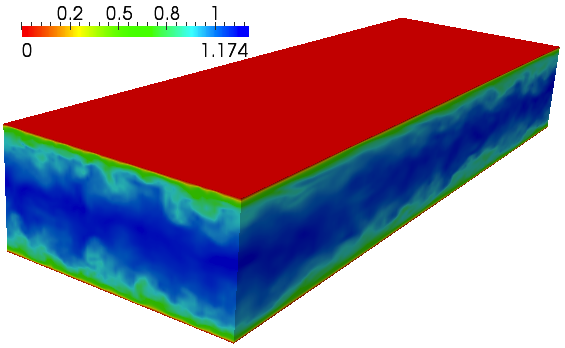
\includegraphics[width=12cm]{Figures/ChanCont.png}
\caption{Velocity profile of the turbulent channel flow (quasi-3D).}
\end{center}
\end{figure}



\subsection{Stability analysis simulations}

Hydrodynamic stability is an important part of fluid-mechanics that has a relevant role in understanding how an unstable flow can evolve into a turbulent state of motion with chaotic three-dimensional vorticity fields and a broad spectrum of small temporal and spatial scales. The essential problems of hydrodynamic stability were recognised and formulated in 19th century, notably by Helmholtz, Kelvin, Rayleigh and Reynolds.

Conventional linear stability assumes a normal representation of the perturbation fields that can be represented as independent wave packets, meaning that the system is self-adjoint. The main aim of the global stability analysis is to evaluate the amplitude of the eigenmodes as time grows and tends to infinity. However, in most industrial applications, it is also interesting to study the behaviour at intermediate states that might affects significantly the functionality and performance of a device. The study of the transient evolution of the perturbations is seen to be strictly related to the non-normality of the linearised Navier-Stokes equations, therefore the normality assumptiong of the system is no longer assumed. The eigenmodes of a non-normal system do not evolve independently and their interaction is responsible for a non-negligible transient growth of the energy. Conventional stability analysis generally does not capture this behaviour, therefore other techniques should be used.

A popular approach to study the hydrodynamic stability of flows consists in performing a direct numerical simulation of the linearised Navier-Stokes equations using iterative methods for computing the solution of the associated eigenproblem. However, since linearly stable flows could show a transient increment of energy, it is necessary to extend this analysis considering the combined effect of the direct and adjoint evolution operators. This phenomenon has noteworthy importance in several engineering applications and it is known as transient growth.

In Nektar++ it is then possible to use the following tools to perform stability analysis: 

\begin{itemize}
\item direct stability analysis;
\item adjoint stability analysis;
\item  transient growth analysis;
\end{itemize}

\subsubsection{Direct stability analysis}


The equations that describe the evolution of an infinitesimal disturbance in the flow can be derived decomposing the solution into a basic state $(\mathbf{U}, p)$ and a perturbed state  $\mathbf{U}+\varepsilon \mathbf{u'}$ with $\varepsilon \ll 1$ that both satisfy the Navier-Stokes equations. Substituting into the Navier Stokes equations and considering that the quadratic terms $\mathbf{u'} \cdot \nabla \mathbf{u'}$can be neglected, we obtain the linearised Navier-Stokes equations:

\begin{subequations}
\begin{equation}
  \frac{\partial \mathbf{u'}}{\partial t} + \mathbf{U} \cdot  \nabla \mathbf{u'}+\mathbf{u'} \cdot \nabla \mathbf{U} = -\nabla p + \nu \nabla^2 \mathbf{u'} + \mathbf{f}
\end{equation}

\begin{equation}
\nabla \cdot \mathbf{u'}
\end{equation}

\end{subequations}



The linearised Navier-Stokes equations are identical in form to the non-linear equation, except for the non-linear advection term. Therefore the numerical techniques used for solving Navier-Stokes equations can still be applied as long as the non-linear term is substituted with the linearised one. It is possible to define the linear operator that evolved the perturbation forward in time:

\begin{equation}
   \mathbf{u'}(\mathbf{x},t)=\mathcal{A}(\mathbf{U})\mathbf{u'}(\mathbf{x},0)
\end{equation}

Let us assume that the base flow  $\mathbf{U}$ is steady, then the perturbations are autonomous and we can assume that:

\begin{equation}
   \mathbf{u'}(\mathbf{x},t)=\mathbf{q'}(\mathbf{x})\exp(\lambda t) \quad \mbox{where} \, \lambda=\sigma+i \omega
\end{equation}

Then we obtain the associated eigenproblem:

\begin{equation}
   \mathcal{A}(\mathbf{U})\mathbf{q'}=\lambda \mathbf{q'}
\end{equation}

The dominant eigenvalue determines the behaviour of the flow. If it the real part is positive there exists exponentially growing solutions, conversely if every single eigenvalues has negative real part then the flow is linearly stable. If the real part of the eigenvalue is zero, it is present a bifurcation point.

\subsubsection{Adjoint Stability Analysis}

The adjoint of a linear operator is one of the most important concept in functional analysis and has an it has important role to tackle the transition to turbulence. Let us write the linearised Navier-Stokes equation in a compact form:

\begin{equation}
\mathcal{H}\mathbf{q}=0 \quad \mbox{where} \quad \mathcal{H}=\left( \begin{array}{c|c}
  -\partial_t-(\mathbf{U} \cdot \nabla)+ (\nabla \mathbf{U}) \cdot + \frac{1}{Re} \nabla^2 & -\nabla \\
  \hline
  \nabla \cdot  & 0
   \end{array}
 \right)
 \end{equation}
 
 
The adjoint operator $(\mathcal{H}^*$ is defines as:

\begin{equation}
\left \langle \mathcal{H}\mathbf{q}, \mathbf{q} \right \rangle= \left \langle \mathbf{q}, \mathcal{H}^*\mathbf{q}^* \right \rangle
\end{equation}

Integrating by parts and employing the divergence theorem, it is possible to express the adjoint equations:

\begin{subequations}
\begin{equation}
-\frac{\partial \mathbf{u}^*}{\partial t}+(\mathbf{U} \cdot \nabla)\mathbf{u}^*+(\nabla \mathbf{U})^T \cdot \mathbf{u}^*=-\nabla p^*+\frac{1}{Re} \nabla^2 \mathbf{u}
\end{equation}

\begin{equation}
\nabla \cdot \mathbf{u}^*=0
\end{equation}
\end{subequations}

The adjoint fields are in fact related to the concept of \textbf{receptivity}. The value of the adjoint velocity at a point in the flow indicates the response that arises from an unsteady momentum source at that point. The adjoint pressure and the adjoint stream function play instead the same role for mass and vorticity sources respectively. Therefore, the adjoint modes can be seen as a powerful tool to understand where to act in order to ease/inhibit the transition.

\subsubsection{Transient Growth Analysis}

Transient growth  is a phenomenon that occurs when a flow that is linearly stable, but whose perturbations exhibit a non-negligible transient response due to regions of localised convective instabilities. This situation is common in many engineering applications, for example in open flows where the geometry is complex, producing a steep variation of the base flow. Therefore, the main question to answer is if it exists a bounded solution that exhibit large growth before inevitably decaying. Let us introduce a norm to quantify the size of a perturbation. It is physically meaningful to use the total kinetic energy of a perturbation on the domain $\Omega$. This is convenient because it is directly associated with the
standard-$L2$ inner product: 

\begin{equation}
\mathcal{A}(\tau)\mathbf{v}=\sigma \mathbf{u}, \quad \left\| \mathbf{u} \right\|=1
\end{equation}


where $\sigma=\left\| \mathbf{u'}(\tau)\right\|$. This is no other that the singular value decomposition of $\mathcal{A}(\tau)$. The phenomenology of the transient growth can be explained considering the non-normality of the linearised Navier-Stokes evolution operator. This can be simply understood using the simple geometric example showed in following figure . Let us assume a unit-length vector $\mathbf{f}$ represented in a non-orthogonal basis .This vector is defined as the difference of the nearly collinear vectors $\mathbf{\Phi_1}$ and $\mathbf{\Phi_2}$.  With the time progression, the component of these two vectors decrease respectively by 20\% and 50\%. The vector $\mathbf{f}$ increases substantially in length before decaying to zero. Thus, the superposition of decaying non-orthogonal eigenmode can produce in short term a growth in the norm of the perturbations. 


\begin{figure}[!htbp]
\centering
 \label{TG}
 {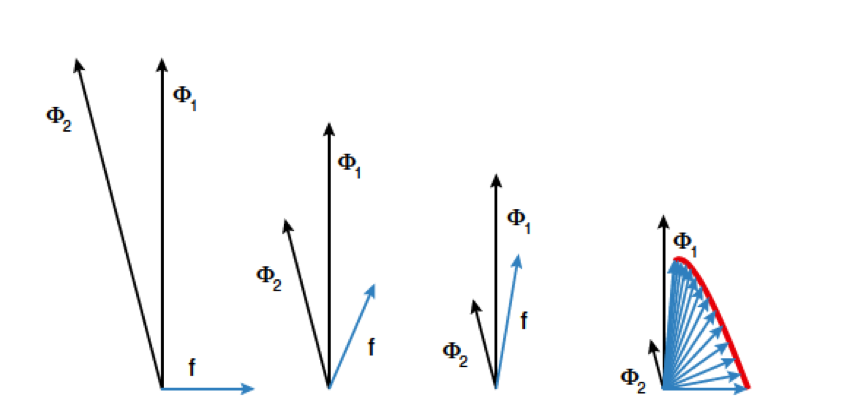
\includegraphics[width=1 \textwidth]{Figures/transient_growth.png}}
   \caption {Geometric interpretation of the transient growth. Adapted from Schmid, 2007 }
\end{figure}

\subsection{Usage}

\texttt {IncNavierStokesSolver session.xml}

\subsection{Session file configuration}

 The type of equation which is to be solved is specified through the \texttt {EquationType} SOLVERINFO option in the session file. This can be set to any of the following: 

\begin{table}
\begin{center}
\begin{tabular}{|l|c|} \hline
{Equation to solve}  \\ \hline
$\frac{\partial\mathbf{u'}}{\partial t} +\mathcal{L}(\mathbf{U},\mathbf{u'})=-\nabla p+\nu \nabla^2 \mathbf{u'}$\\ \hline
\end{tabular}
\end{center}
\end{table}


\begin{table}
\begin{center}
\begin{tabular}{|l|c|c|c|c|c|} \hline
{Equation Type} & {Dimensions} &{Projections} &{Algorithms} \\ \hline
UnsteadyNavierStokes & 2D, Quasi-3D& Continuous &VCS,DS\\ \hline
\end{tabular}
\end{center}
\end{table}

\subsubsection{Solver Info}

\begin{itemize}
\item \texttt{Eqtype}:  sets the type of equation to solve, according to the table above.
\item \texttt{TimeIntegrationMethod}: the following types of time integration methods have been tested with each solver:
\begin{table}
\begin{center}
\begin{tabular}{|l|c|c|c|c|c|} \hline
{} & {Explicit} &{Diagonally Implicit} &{IMEX} & {Implicit} \\ \hline
\texttt{UnsteadyNavierStokes} & X & &X & \\ \hline
\end{tabular}
\end{center}
\end{table}
\end{itemize}

\begin{itemize}
\item \texttt{Projection}: the Galerkin projection used may be either 
\begin{itemize}
\item \texttt{Continuous}: for a C0-continuous Galerkin (CG) projection;
\item \texttt{Discontinuous}: for a discontinous Galerkin (DG) projection. 
\end{itemize}

\item \texttt{EvolutionOperator}:
\begin{itemize}
\item \texttt{Nonlinear} (non-linear Navier-Stokes equations).
\item \texttt{Direct} (linearised Navier-Stokes equations).
\item \texttt{Adjoint} (adjoint Navier-Stokes equations).
\item \texttt{TransientGrowth} ((transient growth evolution operator).
\end{itemize}

\item \texttt{Driver}: specifies  the type of problem to be solved:
   \begin{itemize}
    \item \texttt{Standard} (time integration of the equations)
    \item \texttt{ModifiedArnoldi} (computations of the leading eigenvalues and eigenmodes using modified Arnoldi method)
    \item \texttt{Arpack} (computations of eigenvalues/eigenmodes using Implicitly Restarted Arnoldi Method (ARPACK) ).
    \end{itemize}
    
\item \texttt{ArpackProblemType}: types of eigenvalues to be computed (for Driver Arpack only) 
\begin{itemize}
\item \texttt{LargestMag} (eigenvalues with largest magnitude).
\item \texttt{SmallestMag} (eigenvalues with smallest magnitude). 
\item \texttt{LargestReal} (eigenvalues with largest real part).
\item \texttt{SmallestReal} (eigenvalues with smallest real part). 
\item \texttt{LargestImag} (eigenvalues with largest imaginary part). 
\item \texttt{SmallestIma} (eigenvalues with smallest imaginary part ). 
\end{itemize}    

\item \texttt{Homogeneous}: specifies the Fourier expansion in a third direction (optional) 
\begin{itemize}
\item \texttt{1D} (Fourier spectral method in z-direction).
\end{itemize}
\item \texttt{ModeType}: this specifies the type of the quasi-3D problem to be solved.
\begin{itemize}
\item \texttt{MultipleMode} (stability analysis with multiple modes).
\item \texttt{SingleMode} (BiGlobal Stability Analysis: full-complex mode).
\item \texttt{HalfMode} (BiGlobal Stability Analysis: half-complex mode u.Re v.Re w.Im p.Re).
\end{itemize}
\end{itemize}

\subsubsection{Parameters}

 The following parameters can be specified in the \texttt{PARAMETERS} section of the session file: 
 
 \begin{itemize}
 \item \texttt{Re}: sets the Reynolds number 
 \item \texttt{Kinvis}: sets the kinematic viscosity $\nu$.
 \item \texttt{kdim}: sets the dimension of the Krylov subspace $\kappa$. Can be used in: \texttt{ModifiedArnoldi} and \texttt{Arpack}. Default value: 16.
 \item \texttt{evtol}: sets the tolerance of the eigenvalues. Can be used in: \texttt{ModifiedArnoldi} and \texttt{Arpack}. Default value: $10^{-6}$.
 \item \texttt{nits}: sets the maximum number of iterations. Can be used in: \texttt{ModifiedArnoldi} and \texttt{Arpack}. Default value: 500.
 \item \texttt{LZ}:  sets the length in the spanswise direction $L_z$. Can be used in \texttt{Homogeneous} set to \texttt{1D}. Default value: 1.
 \item \texttt{HomModesZ}: sets the number of planes in the homogeneous directions. Can be used in \texttt{Homogeneous} set to \texttt{1D} and \texttt{ModeType} set to \texttt{MultipleModes}.
  \item \texttt{N\_slices}: sets the number of temporal slices for Floquet stability analysis.
 \item \texttt{period}: sets the periodicity of the base flow. 
 \end{itemize}
 
 \subsubsection{Functions}
 
 \begin{itemize}
 \item To be INserted
 \end{itemize}
 
 \subsection{Examples}
 
 \subsubsection{1. 2D direct stability analysis of the channel flow}
 
  In this example, it will be illustrated how to perform a direct stability analysis using Nektar++. Let us consider a canonical stability problem, the flow in a channel which is confined in the wall-normal direction between two infinite plates (Poiseuille flow) at Reynolds number 7500. This problem is a particular case of the stability solver for the IncNavierStokesSolver. 
  
 \textbf{Background}
 
  We consider the linearised Incompressible Navier-Stokes equations: 
  
  \begin{subequations}
  \begin{equation}
    \frac{\partial \mathbf{u'}}{\partial t} + \mathbf{U} \cdot  \nabla \mathbf{u'}+\mathbf{u'} \cdot \nabla \mathbf{U} = -\nabla p + \nu \nabla^2 \mathbf{u'} + \mathbf{f}
  \end{equation}
  
  \begin{equation}
  \nabla \cdot \mathbf{u'} = 0
  \end{equation}
  \end{subequations}
  
  We are interested to compute the leading eigenvalue of the system using the Arnoldi method.
  
  \textbf{Geometry}
  
   The geometry under consideration is a 2D channel. 
   
   \textbf{Mesh Definition}
   
   In the \texttt{GEOMETRY} section, the dimensions of the problem are defined. Then, the coordinates (\texttt{XSCALE}, \texttt{YSCALE}, \texttt{ZSCALE}) of each vertices of each element are specified. As this input file defines a two-dimensional problem: \texttt{ZSCALE = 0}. 
   
  \begin{lstlisting}[style=XMLStyle]
<GEOMETRY DIM="2" SPACE="2">
        <VERTEX>
            <V ID="0">3.142e+00 1.000e+00 0.000e+00</V>
            ...
            <V ID="62">-3.142e+00 -1.000e+00 0.000e+00</V>
        </VERTEX>
\end{lstlisting}

Edges can now be defined by two vertices.

  \begin{lstlisting}[style=XMLStyle]
<EDGE>
            <E ID="0">    0  1   </E>
            ...
            <E ID="109">   62  55   </E>
        </EDGE>
\end{lstlisting}


In the \texttt{ELEMENT} section, the tag \texttt{T} and \texttt{Q} define respectively triangular and quadrilateral element. Triangular elements are defined by a sequence of three edges and quadrilateral elements by a sequence of four edges.

  \begin{lstlisting}[style=XMLStyle]
        <ELEMENT>
            <Q ID="0">    0     1     2     3 </Q>
            ...
            <Q ID="47">  107   108   109    95 </Q>
        </ELEMENT>
        \end{lstlisting}

Finally, collections of elements are listed in the \texttt{COMPOSITE} section and the \texttt{DOMAIN} section specifies that the mesh is composed by all the triangular and quadrilateral elements. The other composites will be used to enforce boundary conditions. 

  \begin{lstlisting}[style=XMLStyle]
              <COMPOSITE>            
            <C ID="0"> Q[0-47] </C>
            <C ID="1"> E[17,31,44,57,70,83,96,109,0,19,32,45,58,71,84,97] </C> //wall
            <C ID="2"> E[3,6,9,12,15,18] </C>//inflow 
            <C ID="3"> E[98,100,102,104,106,108] </C> //outflow
        </COMPOSITE>
        <DOMAIN> C[0] </DOMAIN>
</GEOMETRY>
  \end{lstlisting}
              
  \textbf{Expansion}
  
  This section defines the polynomial expansions used on each composites. For this example we will use a 10th order polynomial, i.e. $P=11$.
  
  \begin{lstlisting}[style=XMLStyle]
<EXPANSIONS>
     <E COMPOSITE="C[0]" NUMMODES="11" FIELDS="u,v,p" TYPE="MODIFIED" />
</EXPANSIONS>
  \end{lstlisting}
  
  \textbf{Solver Info}
  
  In this example the \texttt{EvolutionOperator} must be \texttt{Direct} to consider the linearised Navier-Stokes equations and the \texttt{Driver} was set up to \texttt{ModifiedArnoldi} for the solution of the eigenproblem. 
  
    \begin{lstlisting}[style=XMLStyle]
      <SOLVERINFO>
      <I PROPERTY="SolverType"        VALUE="VelocityCorrectionScheme"/>
      <I PROPERTY="EQTYPE"            VALUE="UnsteadyNavierStokes"/>
      <I PROPERTY="EvolutionOperator" VALUE="Direct"/>
      <I PROPERTY="Projection"        VALUE="Galerkin"/>
      <I PROPERTY="Driver"            VALUE= "ModifiedArnoldi" />
      <I PROPERTY="TimeIntegrationMethod" VALUE="IMEXOrder1" />    
    </SOLVERINFO>
      \end{lstlisting}


\textbf{Parameters}

All the stability parameters are specified in this section. 

    \begin{lstlisting}[style=XMLStyle]
<PARAMETERS>
      <P> TimeStep      = 0.002 </P>
      <P> NumSteps      = 500 </P>
      <P> IO_CheckSteps = 1000    </P>
      <P> IO_InfoSteps  = 10    </P>
      <P> Re            = 7500     </P>
      <P> Kinvis         =1./Re   </P>
      <P> kdim           =16   </P>
      <P> nvec           =2   </P>
      <P> evtol          =1e-5</P>
      <P> nits           =5000 </P>
   </PARAMETERS>
         \end{lstlisting}
         
         
\textbf{Boundary Conditions}

    \begin{lstlisting}[style=XMLStyle]
 <BOUNDARYREGIONS>
            <B ID="0"> C[1] </B>
            <B ID="1"> C[2] </B>
            <B ID="2"> C[3] </B>
        </BOUNDARYREGIONS>

        <BOUNDARYCONDITIONS>
            <REGION REF="0">
                <D VAR="u" VALUE="0" />
                <D VAR="v" VALUE="0" />
                <N VAR="p" USERDEFINEDTYPE="H" VALUE="0" />
            </REGION>
            <REGION REF="1">
                <P VAR="u" VALUE="[2]" />
                <P VAR="v" VALUE="[2]" />
                <P VAR="p" VALUE="[2]" />
            </REGION>
            <REGION REF="2">
                <P VAR="u" VALUE="[1]" />
                <P VAR="v" VALUE="[1]" />
                <P VAR="p" VALUE="[1]" />
            </REGION>
        </BOUNDARYCONDITIONS>
                 \end{lstlisting}

\textbf{Function}

We need to set up the base flow that can be specified as a function \texttt{BaseFlow}. In case the base flow is not analytical, it can be generated by means of the \texttt{Nonlinear} evolution operator using the same mesh and polynomial expansion. The initial guess is specified in the \texttt{InitialConditions} functions and can be both analytical or a file. In this example it is read from a file. 

    \begin{lstlisting}[style=XMLStyle]
<FUNCTION NAME="BaseFlow">
            <F VAR="u,v,p" FILE="ChanStability.bse" />
        </FUNCTION>

        <FUNCTION NAME="InitialConditions">
            <F VAR="u,v,p" FILE="ChanStability.rst" />
        </FUNCTION>
                         \end{lstlisting}



\textbf{Usage}

\texttt{IncNavierStokesSolver ChanStability.xml}


\textbf{Results}

The stability simulation takes about 250 iterations to converge and the dominant eigenvalues (together with the respective eigenvectors) will be printed. In this case it was found $    \lambda_{1,2}=1.000224 \times e^{\pm 0.24984i}$. Therefore, since the magnitude of the eigenvalue is larger than 1, the flow is absolutely unstable. It is possible to visualise the eigenvectors using the post-processing utilities. The figure shows the profile of the two eigenmode component, which shows the typical Tollmien - Schlichting waves that arise in viscous boundary layers.

\begin{figure}[!htbp]
\centering
 {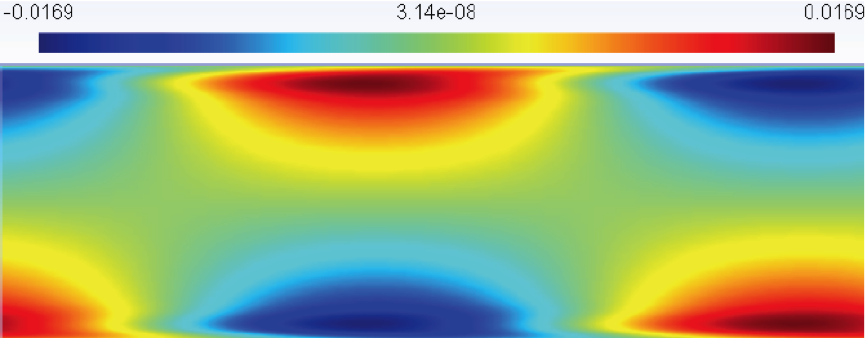
\includegraphics[width=1 \textwidth]{Figures/chan_u.png}}
   \caption {}
\end{figure}

\begin{figure}[!htbp]
\centering
 {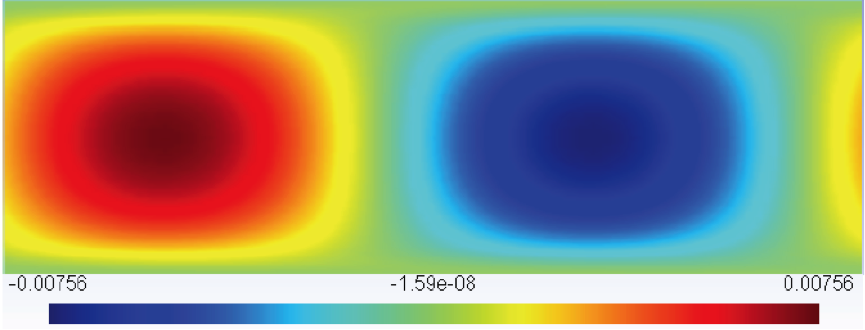
\includegraphics[width=1 \textwidth]{Figures/chan_v}}
    \caption {}
\end{figure}

 \subsubsection{2. 2D adjoint stability analysis of the channel flow}

 In this example, it will be illustrated how to perform an adjoint stability analysis using Nektar++. Let us consider a canonical stability problem, the flow in a channel which is confined in the wall-normal direction between two infinite plates (Poiseuille flow) at Reynolds number 7500
 
 \textbf{Background}
 
  We consider the equations: 
  
  \begin{subequations}
  \begin{equation}
  -\frac{\partial \mathbf{u}^*}{\partial t}+(\mathbf{U} \cdot \nabla)\mathbf{u}^*+(\nabla \mathbf{U})^T \cdot \mathbf{u}^*=-\nabla p^*+\frac{1}{Re} \nabla^2 \mathbf{u}
  \end{equation}
  
  \begin{equation}
  \nabla \cdot \mathbf{u}^*=0
  \end{equation} 
  \end{subequations}
  
  We are interested in computing the leading eigenvalue of the system using the Arnoldi method.
  
 \textbf{Geometry \& Mesh}
 
 The geometry and mesh are the same ones used for the direct stability analysis in the previous example.
 
 \textbf{Solver Info}
 
 This sections defines the problem solved. In this example the \texttt{EvolutionOperator} must be \texttt{Adjoint} to consider the adjoint Navier-Stokes equations and the \texttt{Driver} was set up to \texttt{ModifiedArnoldi} for the solution of the eigenproblem. 

    \begin{lstlisting}[style=XMLStyle]
<SOLVERINFO>
      <I PROPERTY="SolverType"        VALUE="VelocityCorrectionScheme"/>
      <I PROPERTY="EQTYPE"            VALUE="UnsteadyNavierStokes"/>
      <I PROPERTY="EvolutionOperator" VALUE="Adjoint"/>
      <I PROPERTY="Projection"        VALUE="Galerkin"/>
      <I PROPERTY="Driver"            VALUE= "ModifiedArnoldi" />
      <I PROPERTY="TimeIntegrationMethod" VALUE="IMEXOrder1" />    
</SOLVERINFO>
  \end{subequations}

\textbf{Parameters}

    \begin{lstlisting}[style=XMLStyle]
<PARAMETERS>
      <P> TimeStep      = 0.002 </P>
      <P> NumSteps      = 500 </P>
      <P> IO_CheckSteps = 1000    </P>
      <P> IO_InfoSteps  = 10    </P>
      <P> Re            = 7500     </P>
      <P> Kinvis         =1./Re   </P>
      <P> kdim           =16   </P>
      <P> nvec           =2   </P>
      <P> evtol          =1e-5</P>
      <P> nits           =5000 </P>
</PARAMETERS>
  \end{lstlisting}

\textbf{Boundary Conditions}

    \begin{lstlisting}[style=XMLStyle]
 <BOUNDARYREGIONS>
            <B ID="0"> C[1] </B>
            <B ID="1"> C[2] </B>
            <B ID="2"> C[3] </B>
        </BOUNDARYREGIONS>

        <BOUNDARYCONDITIONS>
            <REGION REF="0">
                <D VAR="u" VALUE="0" />
                <D VAR="v" VALUE="0" />
                <N VAR="p" USERDEFINEDTYPE="H" VALUE="0" />
            </REGION>
            <REGION REF="1">
                <P VAR="u" VALUE="[2]" />
                <P VAR="v" VALUE="[2]" />
                <P VAR="p" VALUE="[2]" />
            </REGION>
            <REGION REF="2">
                <P VAR="u" VALUE="[1]" />
                <P VAR="v" VALUE="[1]" />
                <P VAR="p" VALUE="[1]" />
            </REGION>
        </BOUNDARYCONDITIONS>
  \end{lstlisting}


\textbf{Functions}

We need to set up the base flow that can be specified as a function \texttt{BaseFlow}. In case the base flow is not analytical, it can be generated by means of the \texttt{Nonlinear} evolution operator using the same mesh and polynomial expansion.

    \begin{lstlisting}[style=XMLStyle]
        <FUNCTION NAME="BaseFlow">
            <F VAR="u,v,p" FILE="ChanStability.bse" />
        </FUNCTION>
  \end{lstlisting}
  
  The initial guess is specified in the \texttt{InitialConditions} functions and can be both analytical or a file. In this example it is read from a file. 
  
      \begin{lstlisting}[style=XMLStyle]
        <FUNCTION NAME="InitialConditions">
            <F VAR="u,v,p" FILE="ChanStability.rst" />
        </FUNCTION>
          \end{lstlisting}

\textbf{Usage}

\texttt{IncNavierStokesSolver ChanStability\_adj.xml}

\textbf{Results}

The equations will then be evolved backwards in time (consistently with the negative sign in front of the time derivative) and the leading eigenvalues will be computed after about 300 iterations. It is interesting to note that their value is the same one computed for the direct problem, but the eigenmodes present a different shape.


\begin{figure}[!htbp]
\centering
 {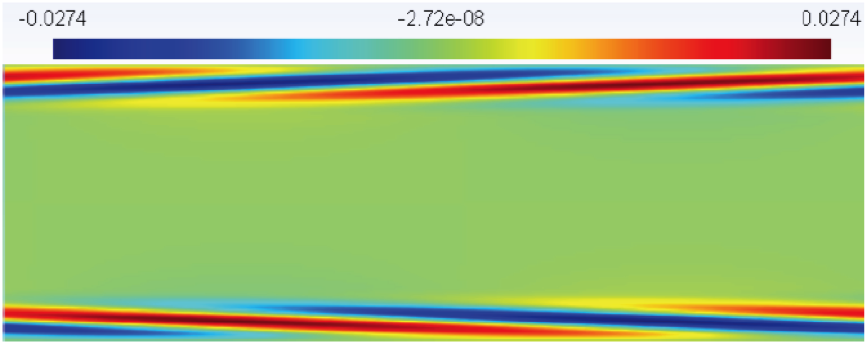
\includegraphics[width=1 \textwidth]{Figures/chan_u_adj.png}}
   \caption {}
\end{figure}

\begin{figure}[!htbp]
\centering
 {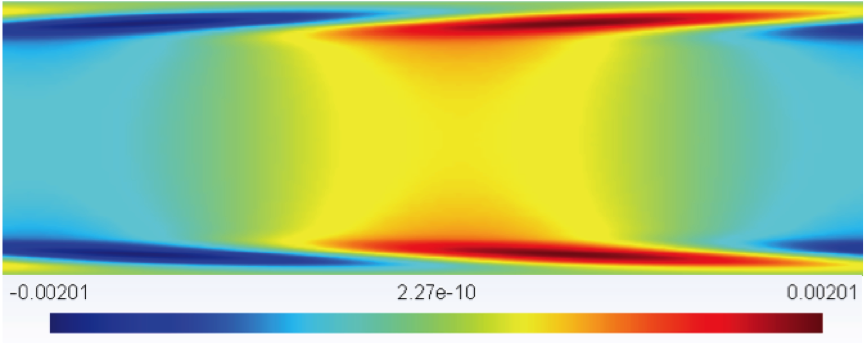
\includegraphics[width=1 \textwidth]{Figures/chan_v_adj}}
    \caption {}
\end{figure}

\subsubsection{3.  2D Transient Growth analysis of a flow past a backward-facing step}

In this section it will be described how to perform a transient growth stability analysis using Nektar++. Let us consider a flow past a backward-facing step (figure \ref{bfs_geo}). This is an important case because it allows us to understand  the effects of separation caused by abrupt changes in the geometry and it is a common geometry in several studies of flow control and turbulence of separated flow.

\begin{figure}[!htbp]
\centering
 {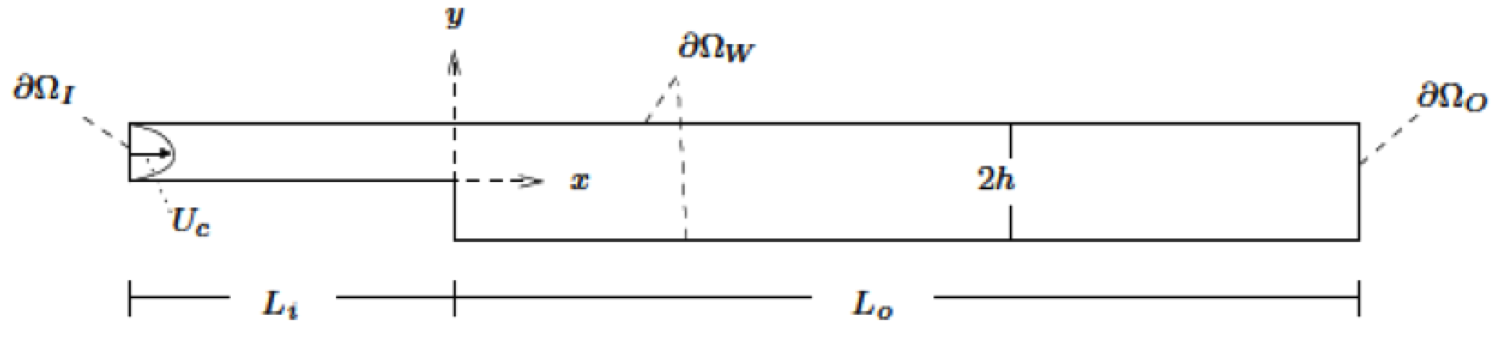
\includegraphics[width=1 \textwidth]{Figures/bfs_geo}}
    \caption {}\label{bfs_geo}
\end{figure}

\textbf{Background}

Transient growth analysis allows us to study the presence of convective instabilities that can arise in stable flows. Despite the fact that these instabilities will decay for a long time (due to the stability of the flow), they can produce significant increases in the energy of perturbations. The phenomenon of transient growth is associated with the non-normality of the linearised Navier-Stokes equations and it consists in computing the perturbation that leads to the highest energy growth for a fixed time horizon.

\textbf{Input Parameters}

In the \texttt{GEOMETRY} section, the dimensions of the problem are defined. Then, the coordinates (\texttt{XSCALE}, \texttt{YSCALE}, \texttt{ZSCALE}) of each vertices are specified. As this input file defines a two-dimensional problem: \texttt{ZSCALE = 0}.

      \begin{lstlisting}[style=XMLStyle]
<GEOMETRY DIM="2" SPACE="2">
   <VERTEX>
       <V ID="0">3.000e+00 -1.000e+00 0.000e+00</V>
       ...
       <V ID="399">-1.000e+01 0.000e+00 0.000e+00</V>
   </VERTEX>
     \end{lstlisting}

Edges can now be defined by two vertices.

      \begin{lstlisting}[style=XMLStyle]
<EDGE>
       <E ID="0">    0  1   </E>
       ...
       <E ID="828">  399  394   </E>
   </EDGE>
        \end{lstlisting}

In the \texttt{ELEMENT} section, the tag \texttt{T} and \texttt{Q} define respectively triangular and quadrilateral element. Triangular elements are defined by a sequence of three edges and quadrilateral elements by a sequence of four edges.

      \begin{lstlisting}[style=XMLStyle]
<ELEMENT>
       <T ID="0">    0     1     2 </T>
       ...
       <T ID="209">  333   314   332 </T>
       <Q ID="210">  334   335   336     0 </Q>
       ...
       <Q ID="429">  826   827   828   818 </Q>
   </ELEMENT>
        \end{lstlisting}

Finally, collections of elements are listed in the \texttt{COMPOSITE} section and the \texttt{DOMAIN} section specifies that the mesh is composed by all the triangular and quadrilateral elements. The other composites will be used to enforce boundary conditions.

      \begin{lstlisting}[style=XMLStyle]
<COMPOSITE>
       <C ID="0"> T[0-209] </C>
       <C ID="1"> Q[210-429] </C>
       <C ID="2"> E[2-3,7,10,16,21,2,...,828] </C>
       <C ID="3"> E[821,823,825,827] </C>
       <C ID="4"> E[722,724,726,728] </C>
   </COMPOSITE>
   
   <DOMAIN> C[0,1] </DOMAIN>
</GEOMETRY>
        \end{lstlisting}

\textbf{Expansion}

For this example we will use a 6th order polynomial, i.e. $P=7$:

      \begin{lstlisting}[style=XMLStyle]
<EXPANSIONS>
    <E COMPOSITE="C[0]" NUMMODES="7" FIELDS="u,v,p" TYPE="MODIFIED" />
    <E COMPOSITE="C[1]" NUMMODES="7" FIELDS="u,v,p" TYPE="MODIFIED" />
</EXPANSIONS> 
        \end{lstlisting}

\textbf{Solver Information}

This sections defines the problem solved. In this example the \texttt{EvolutionOperator} must be \texttt{TransientGrowth} and the \texttt{Driver} was set up to \texttt{Arpack} for the solution of the eigenproblem. 

      \begin{lstlisting}[style=XMLStyle]
 <SOLVERINFO>
            <I PROPERTY="EQTYPE"                VALUE="UnsteadyNavierStokes"    />
            <I PROPERTY="EvolutionOperator"     VALUE="TransientGrowth"         />
            <I PROPERTY="Projection"            VALUE="Galerkin"                />
            <I PROPERTY="TimeIntegrationMethod" VALUE="IMEXOrder2"              />
            <I PROPERTY="SOLVERTYPE"            VALUE="VelocityCorrectionScheme"/>
            <I PROPERTY="Driver"                VALUE="Arpack"                  />
            <I PROPERTY="ArpackProblemType"     VALUE="LargestMag"              />
        </SOLVERINFO>
                \end{lstlisting}


\textbf{Parameters}

      \begin{lstlisting}[style=XMLStyle]
<PARAMETERS>
            <P> FinalTime       = 0.1                   </P>
            <P> TimeStep        = 0.005                 </P>
            <P> NumSteps        = FinalTime/TimeStep    </P>
            <P> IO_CheckSteps   = 1/TimeStep            </P>
            <P> IO_InfoSteps    = 1                     </P>
            <P> Re              = 500                   </P>
            <P> Kinvis          = 1.0/Re                </P>
            <P> kdim            = 4                     </P>
            <P> nvec            = 1                     </P>
            <P> evtol           = 1e-4                  </P>
        </PARAMETERS>
                        \end{lstlisting}
                        
                        
\textbf{Boundary Conditions}

      \begin{lstlisting}[style=XMLStyle]
 <BOUNDARYREGIONS>
            <B ID="0"> C[2] </B>    <!-- Wall -->
            <B ID="1"> C[3] </B>    <!-- Inlet -->
            <B ID="2"> C[4] </B>    <!-- Outlet -->
        </BOUNDARYREGIONS>

        <BOUNDARYCONDITIONS>
            <REGION REF="0">
                <D VAR="u" VALUE="0" />
                <D VAR="v" VALUE="0" />
                <N VAR="p" USERDEFINEDTYPE="H" VALUE="0" />
            </REGION>
            <REGION REF="1">
                <D VAR="u" VALUE="0" />
                <D VAR="v" VALUE="0" />
                <N VAR="p" USERDEFINEDTYPE="H" VALUE="0" />
            </REGION>
            <REGION REF="2">
                <D VAR="u" VALUE="0" />
                <D VAR="v" VALUE="0" />
                <N VAR="p" USERDEFINEDTYPE="H" VALUE="0" />
            </REGION>
        </BOUNDARYCONDITIONS>
                                \end{lstlisting}

\textbf{Functions}

We need to set up the base flow that can be specified as a function \texttt{BaseFlow}. In case the base flow is not analytical, it can be generated by means of the \texttt{Nonlinear} evolution operator using the same mesh and polynomial expansion.

      \begin{lstlisting}[style=XMLStyle]
<FUNCTION NAME="BaseFlow">
            <F VAR="u,v,p" FILE="bfs_tg-AR.bse" />
        </FUNCTION>
                                        \end{lstlisting}


The initial guess is specified in the \texttt{InitialConditions} functions and in this case is read from a file. 
 
 \begin{lstlisting}[style=XMLStyle]  
<FUNCTION NAME="InitialConditions">
            <F VAR="u,v,p" FILE="bfs_tg-AR.rst" />
        </FUNCTION>
                                        \end{lstlisting}


\textbf{Usage}

\texttt{IncNavierStokesSolver bfs\_tg-AR.xml}

\textbf{Results}

The solution will be evolved forward in time using the operator $\mathcal{A}$, then backward in time through the adjoint operator $\mathcal{A}^*$. The leading eigenvalue is $\lambda= 3.236204)$. This corresponds to the largest possible transient growth at the time horizon $\tau= 1$. The leading eigenmode is shown below. This is the optimal initial condition which will lead to the greatest growth when evolved under the linearised Navier-Stokes equations.


\begin{figure}[!htbp]
\centering
 {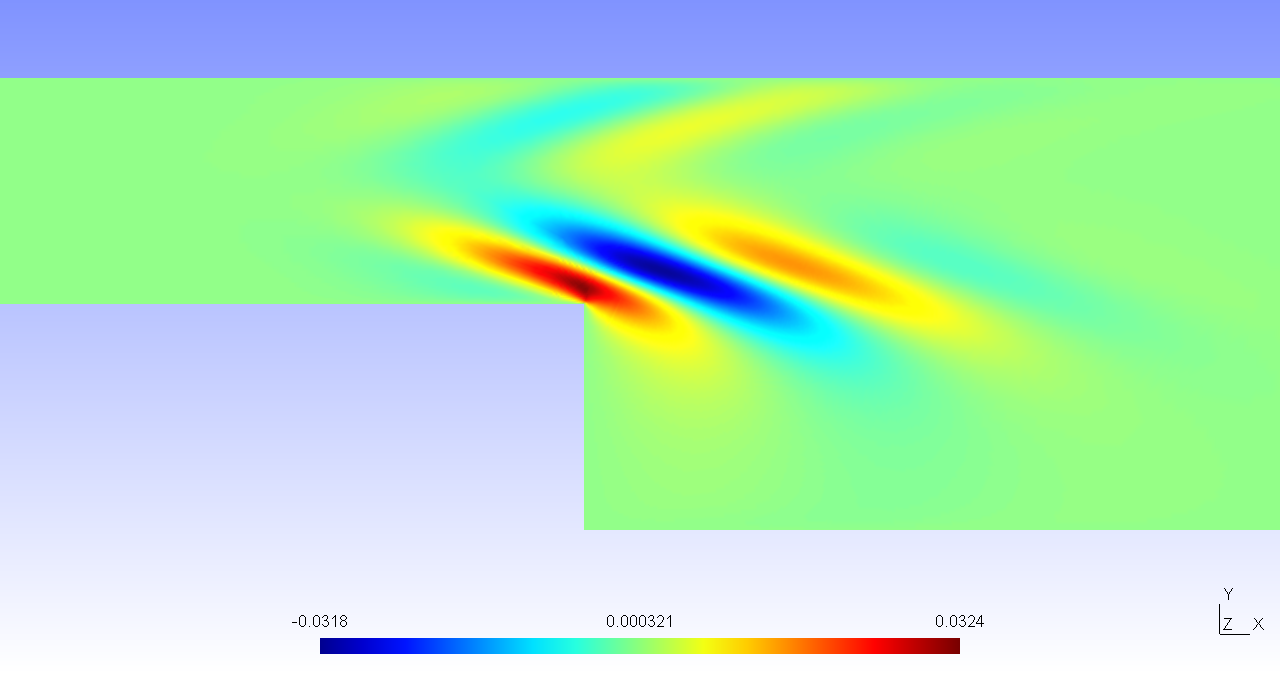
\includegraphics[width=1 \textwidth]{Figures/bfs_eig_u}}
   \caption {}
\end{figure}

\begin{figure}[!htbp]
\centering
 {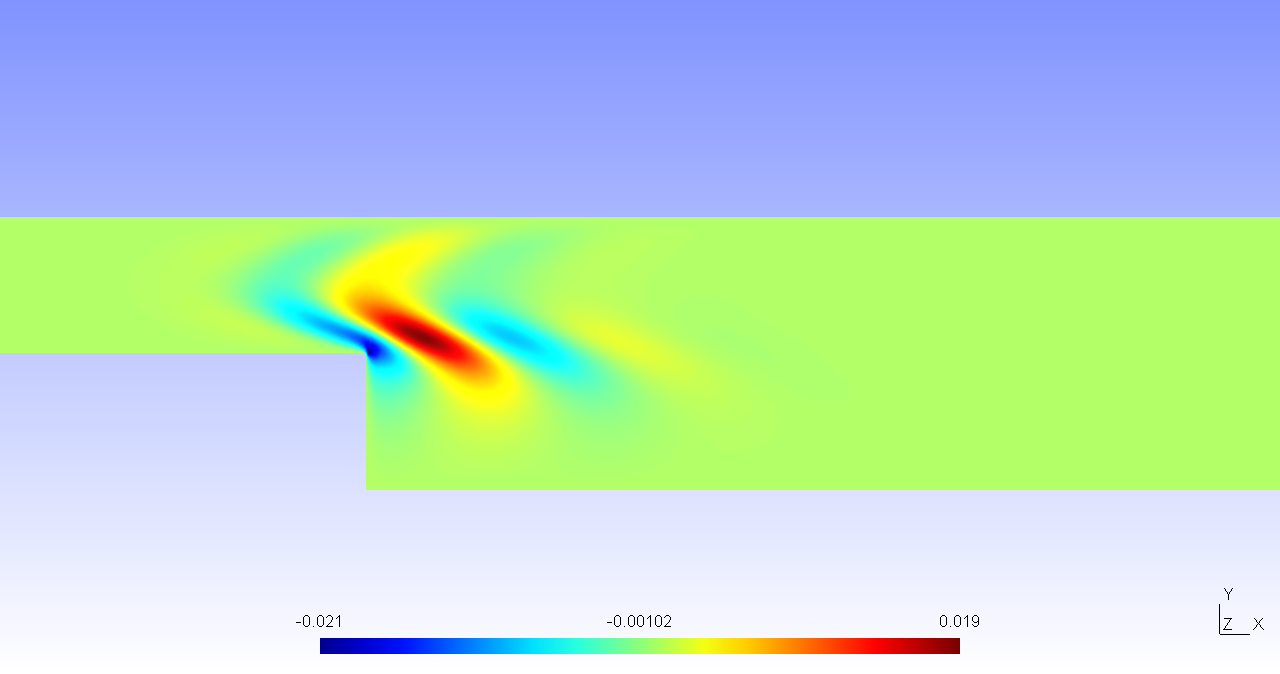
\includegraphics[width=1 \textwidth]{Figures/bfs_eig_v}}
    \caption {}
\end{figure}

It is possible to visualise the transient growth plotting the energy evolution over time if the system is initially perturbed with the leading eigenvector. This analysis was performed  for a time horizon $\tau= 60$. It can be seen that the energy grows in time reaching its maximum value at x = 24 and then decays, almost disappearing after 100 temporal units.


\begin{figure}[!htbp]
\centering
 {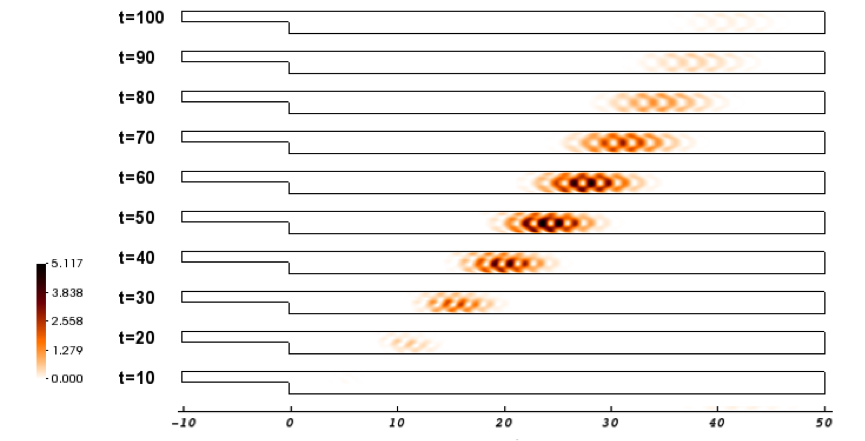
\includegraphics[width=1 \textwidth]{Figures/energy_bfs}}
   \caption {}
\end{figure}

\textbf{4. BiGlobal Floquet analysis of a of flow past a cylinder}

 In this example it will be described how to run a BiGlobal stability analysis for a time-periodic base flow using Nektar++. Let us consider a flow past a circular cylinder at $Re=220$ has a 2D time-periodic wake that is unstable to a 3D synchronous "mode A" instability. 
 
 \begin{figure}[!htbp]
\centering
 {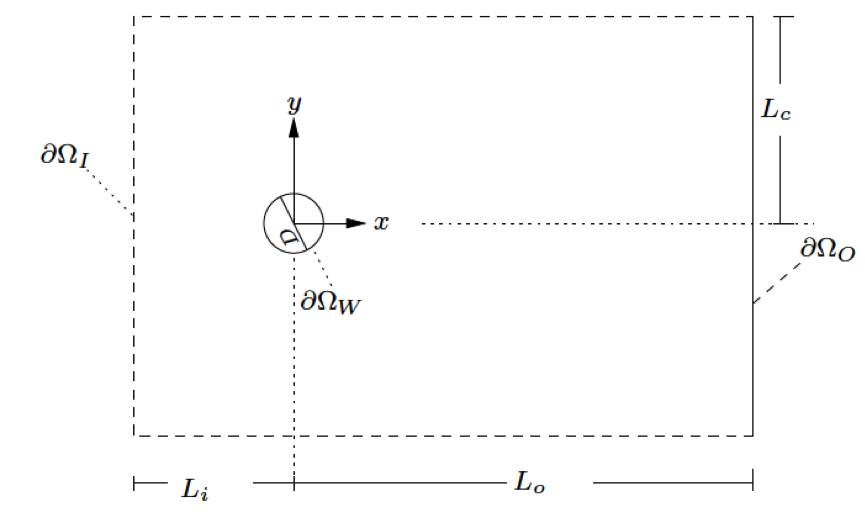
\includegraphics[width=1 \textwidth]{Figures/cylinder_geo}}
   \caption {}
\end{figure}

  
\textbf{Background}

The numerical solution of the fully three- dimensional linear eigenvalue problem is often computationally demanding and may not have significant advantages over performing a direct numerical simulation. Therefore, some simplifications are required; the most radical consist in considering that the base flow depends only on one spatial coordinate, assuming that the other two spatial coordinates are homogenous.  While this method offers a good prediction for the instability of boundary layers, it is not able to predict the instability of Hagen-Poiseuille flow in a pipe at all Reynolds numbers.  Between a flow that depends upon one and three-spatial directions, it is possible to consider a steady or time-periodic base flow depending upon two spatial directions and impose three-dimensional disturbances that are periodic in the the third homogeneous  spatial direction. This approach is known as BiGlobal stability analysis and it represents the extension of the classic linear stability theory; let us consider a base flow $\mathbf{U}$ that is function of only two spatial coordinates: $mathbf{U}(x, y,t)$. The perturbation velocity can $\mathbf{u'}$ can be expressed in a similar form, but with the dependence on the third homogeneous direction incorporated through the Fourier mode: $\mathbf{u'}=\mathbf{\hat{u}'}(x, y, t) e^{i \beta z}$, where $\beta=2\pi/L)$and $L$ is the length in the homogeneous direction.

\textbf{Input parameters}

In this example we use a mesh of 500 quadrilateral elements with a 6th order polynomial expansion. The base flow has been computed using the \texttt{Nonlinear} evolution operator with appropriate boundary conditions. From its profile, it was possible to determine the periodicity of the flow sampling the velocity profile over time. In order to reconstruct the temporal behaviour of the flow, 32 time slices were considered over one period. Using these data it is possible to set up the stability simulation for a specified $\beta$, for example $\beta=1.7$. Let us note that while the base flow is 2D, the stability simulation that we are performing is 3D.

\textbf{Expansion}

In this example we will use a 6th order polynomial expansion, i.e. $P=7$.

 \begin{lstlisting}[style=XMLStyle]  
<EXPANSIONS>
        <E COMPOSITE="C[0]" NUMMODES="7" TYPE="GLL_LAGRANGE_SEM" FIELDS="u,v,w,p" />
    </EXPANSIONS> 
                                            \end{lstlisting}
                                            
                                            
\textbf{Parameters}

 \begin{lstlisting}[style=XMLStyle]  
<SOLVERINFO>
      <I PROPERTY="SolverType"        VALUE="VelocityCorrectionScheme"/>
      <I PROPERTY="EQTYPE"            VALUE="UnsteadyNavierStokes"/>
      <I PROPERTY="EvolutionOperator" VALUE="Direct"/>
      <I PROPERTY="Projection"        VALUE="Galerkin"/>
      <I PROPERTY="ModeType"          VALUE="HalfMode"/>
      <I PROPERTY="Driver"            VALUE= "ModifiedArnoldi" />
      <I PROPERTY="HOMOGENEOUS"       VALUE="1D"/>
      <I PROPERTY="TimeIntegrationMethod" VALUE="IMEXOrder2" />  
</SOLVERINFO>
                                            \end{lstlisting}


\textbf{Functions}

 \begin{lstlisting}[style=XMLStyle]  
<FUNCTION NAME="BaseFlow">
      <F VAR="u,v,p" FILE="cyinder_floq" />
</FUNCTION>
                                            \end{lstlisting}


  \textbf{Usage}
  
\texttt{IncNavierStokesSolver session.xml}

\textbf{Results}

The stability simulation takes about 20 cycles to converge and the leading eigenvalue is $\lambda=1.2670$ with a growth rate $\sigma=4.7694e-02$. The figure below shows the profile of the magnitude of the eigenmode at $z=2$.

\begin{figure}[!htbp]
\centering
 {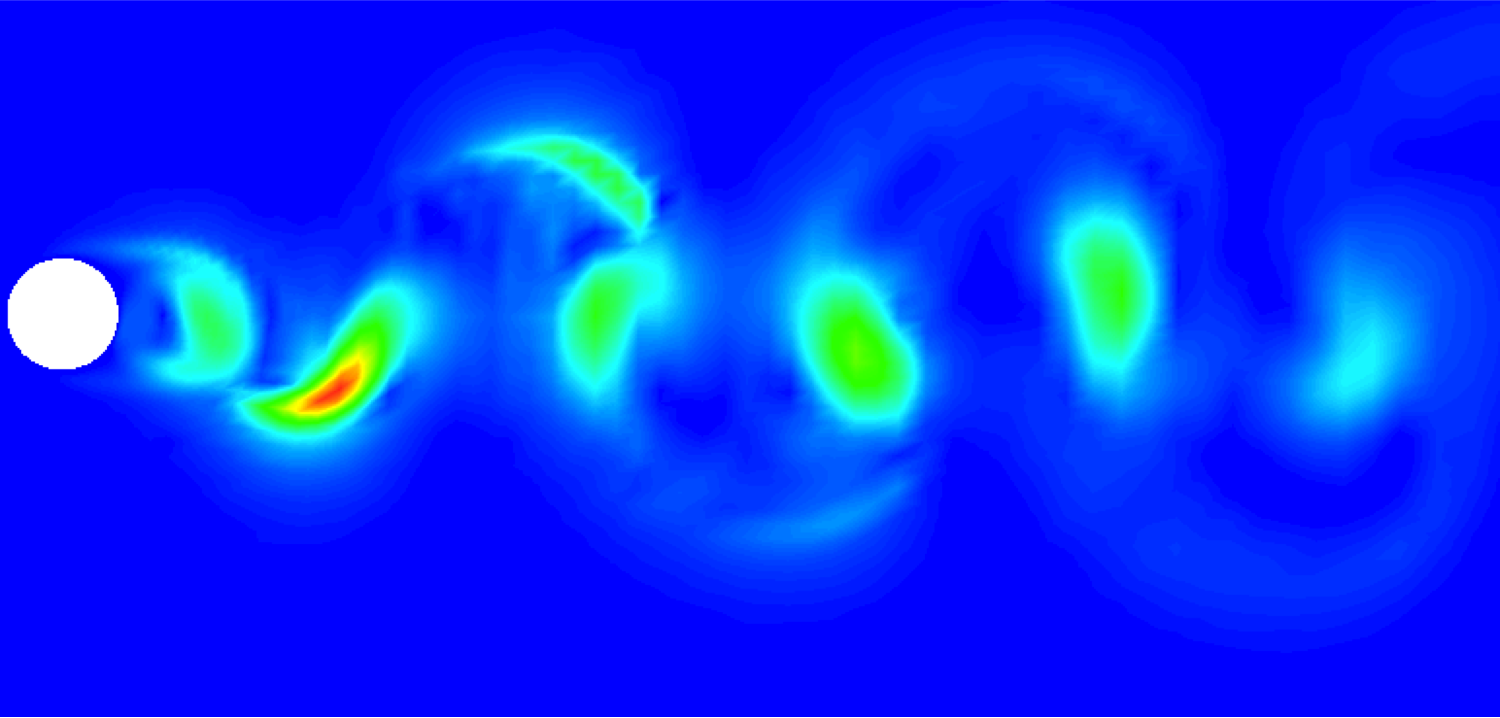
\includegraphics[width=1 \textwidth]{Figures/floquet}}
   \caption {}
\end{figure}

